\documentclass[a4paper]{article}
\usepackage[czech]{babel}
\usepackage[T1]{fontenc} 
\usepackage{amsmath}
\usepackage{titlesec}
\usepackage{amsfonts}
\usepackage[hypcap=false]{caption}
\usepackage[unicode]{hyperref}
\usepackage{tabularx}
\usepackage[nottoc,numbib]{tocbibind}
\usepackage{listings}
\usepackage{color}
\usepackage{inputenc}
\usepackage{textcomp}
\usepackage{xcolor}
\usepackage{newverbs}[2010/09/02]
\usepackage{graphicx}
\usepackage{makecell}
\usepackage[normalem]{ulem}

\renewcommand{\lstlistingname}{Ukázka kódu}
\renewcommand{\lstlistlistingname}{Seznam ukázek kódu}

\definecolor{codegreen}{rgb}{0,0.6,0}
\definecolor{codegray}{rgb}{0.5,0.5,0.5}
\definecolor{codepurple}{rgb}{0.58,0,0.82}

\lstdefinestyle{pythonstyle}{
    backgroundcolor=\color{white},   
    commentstyle=\color{codegreen},
    keywordstyle=\color{blue},
    numberstyle=\tiny\color{codegray},
    stringstyle=\color{codepurple},
    basicstyle=\ttfamily\footnotesize,
    breaklines=true,                 
    captionpos=b,
    numbers=left,                    
    numbersep=5pt,                  
    tabsize=4,
    frame=single 
}

\lstdefinestyle{htmlstyle}{
    language=HTML,
    backgroundcolor=\color{white},   
    commentstyle=\color{codegreen},
    keywordstyle=\color{blue},
    numberstyle=\tiny\color{codegray},
    stringstyle=\color{codepurple}, 
    basicstyle=\ttfamily\footnotesize,
    breaklines=true,                 
    captionpos=b,                    
    numbers=left,                    
    numbersep=5pt,                  
    tabsize=4,
    frame=single,
    alsodigit={.-},
    morekeywords={doctype, html, head, title, body, div, span, h1, p, a, img, script, style},
    tagstyle=\color{blue},
    emph={id, class, src, href, alt, rel, type, target}, 
    emphstyle=\color{blue} 
}

\lstset{style=pythonstyle}

\renewcommand{\refname}{Bibliografie}
\addto\captionsczech{\renewcommand{\refname}{Bibliografie}}


\titleformat{\section}{\huge\bfseries}{\thesection}{1em}{}
\titleformat{\subsection}{\Large\bfseries}{\thesubsection}{1em}{}

\title{Strojové učení v~energetice: Predikce cen elektřiny na~denním trhu}
\author{Jiří Stodůlka}

\begin{document}
\begin{titlepage}
    \centering
    {\large
    \textbf{STŘEDOŠKOLSKÁ ODBORNÁ ČINNOST}\\
    \textbf{Obor č. 18: Informatika}}

    \vspace*{\fill}

    {\Huge \textbf{Strojové učení v~energetice: \\ Predikce cen elektřiny na~denním trhu}\par}
    
    \vspace*{\fill}
    
    \large
    \noindent
    \textbf{
    \begin{flushleft}
        Jiří Stodůlka \\
        Zlínský kraj \hfill Zlín 2026
    \end{flushleft}
    }

\end{titlepage}

\begin{titlepage}

    {\centering
    {\large
    \textbf{STŘEDOŠKOLSKÁ ODBORNÁ ČINNOST}\\
    \textbf{Obor č. 18: Informatika}}

    \vspace*{\fill}

    {\Huge \textbf{Strojové učení v~energetice: \\ Predikce cen elektřiny na~denním trhu}\par}
    {\Huge \textbf{\\Machine Learning \\ in the Energy Sector: Electricity Price Prediction on the Day-Ahead Market}\par}
    }
    \vspace*{\fill}
    {\large
    \noindent
    \textbf{Autor:} Jiří Stodůlka\\
    \textbf{Škola:} Gymnázium a~Jazyková škola s~právem státní jazykové zkoušky Zlín, nám.~T.~G~Masaryka 2734, 760~01~Zlín\\
    \textbf{Kraj:} Zlínský kraj\\
    \textbf{Konzultant:} Mgr.~Michal~Mikláš\\[5mm]
    Zlín 2026}

\end{titlepage}
\section*{Prohlášení}
Prohlašuji, že jsem svou práci SOČ vypracoval samostatně a~použil jsem pouze prameny a~literaturu uvedené v~seznamu bibliografických záznamů.

Beru na vědomí, že nejpozději odevzdáním slovesné vědecké práce do veřejné soutěže Středoškolská odborná činnost, stejně jako odevzdáním jejích příloh a~dalších připojených děl, např. audiovizuálních, fotografických, výtvarných, architektonických apod. (dále jen „soutěžní dílo“), dochází ke zveřejnění díla podle § 4 odst. 1 zákona č. 121/2000 Sb., autorského zákona, ve znění pozdějších předpisů (dále jen „autorský zákon“). Totéž platí pro pozdější odevzdání doplněného, změněného, upraveného nebo opraveného díla. 

Beru na vědomí, že zveřejněním díla, jehož součástí je vynález, se tento vynález stává součástí stavu techniky podle § 5 odst. 1, 2 zákona č. 527/1990 Sb., o~vynálezech, průmyslových vzorech a~zlepšovacích návrzích, ve znění pozdějších předpisů (dále jen „patentový zákon“), což zakládá překážku pro udělení patentu podle § 3 odst. 1 patentového zákona.

Beru na vědomí, že vyhlašovatel soutěže je podle § 61 odst. 1 autorského zákona per analogiam oprávněn užít soutěžní dílo pro účely zajištění průběhu soutěže, zejména k~zajištění transparentnosti soutěže a~veřejnosti obhajob soutěžních prací. V~odůvodněném rozsahu je tedy vyhlašovatel po dobu účasti autora v~soutěži oprávněn zejména:

\begin{itemize}
    \item zhotovovat rozmnoženiny díla, je-li to nezbytné k~seznámení účastníků soutěže, porotců nebo veřejnosti se soutěžní prací; 

    \item zapůjčit originál nebo rozmnoženinu díla účastníkům soutěže, porotcům nebo veřejnosti. Přitom dbá na bezpečné nakládání s~dílem; 

    \item vystavovat originál nebo rozmnoženinu díla v~průběhu soutěžních přehlídek a~doprovodných akcí;  

    \item sdělovat dílo veřejnosti v~nehmotné podobě, a~to především počítačovou nebo obdobnou sítí. 
\end{itemize}

Dále prohlašuji, že při tvorbě této práce jsem použil nástroj generativního modelu AI (Google Gemini; gemini.google.com) za účelem kontroly gramatiky a~reformulace textu. Po použití tohoto nástroje jsem provedl kontrolu obsahu a~přebírám za něj plnou zodpovědnost.\\[3cm] 

\noindent Ve~Zlíně dne 11.~3.~2026~\dotuline{Jiří Stodůlka}
\newpage

\section*{Poděkování}
V~první řadě bych chtěl poděkovat svému tátovi, bez něj by tato práce vůbec nevznikla. Právě on mě zasvětil do základních principů trhu s~elektřinou, což bylo pro pochopení celého tématu klíčové. Dále bych také rád poděkoval panu učiteli informatiky Mgr.~Michalu~Miklášovi, bez jeho pobízení a~motivace bych se do soutěže vůbec nepřihlásil. 
\newpage

\section*{Anotace}
Tato práce se zabývá návrhem a~implementací modelu strojového učení pro predikci cen elektřiny na českém denním trhu (organizovaném společností OTE,~a.s.). Cílem bylo prozkoumat, jak přesných výsledků lze dosáhnout za použití pouze veřejně dostupných dat. V~rámci projektu byla shromážděna datová sada zahrnující historické tržní ceny, data o~spotřebě a~údaje o~výrobě obnovitelných zdrojů. Pro snadnou vizualizaci výsledků a~jejich porovnání se skutečnými cenami bylo nad modelem postaveno webové rozhraní. Projekt demonstruje schopnost projít celým životním cyklem data science projektu~-- od sběru veřejných dat, přes trénink modelu, až po jeho nasazení a~vizualizaci pro koncového uživatele.

\section*{Klíčová slova}
strojové učení, predikce cen elektřiny, denní trh, vizualizace dat, dataset, webová aplikace.

\section*{Annotation}
This project focuses on the design and implementation of a~machine learning model for predicting electricity prices on the Czech day-ahead market (organized by OTE,~a.s.). The aim was to explore the level of prediction accuracy achievable using solely publicly available data. As part of the project, a~comprehensive dataset was compiled, composed of historical market prices, electricity consumption data, and renewable energy generation data. To provide straightforward visualization of the results and their comparison with actual prices, a~web interface was built on top of the model. The project demonstrates the ability to execute the entire data science project lifecycle~-- from collecting public data and training the model, through to its deployment and visualization for the end user.
\section*{Keywords}
machine learning, electricity price prediction, day-ahead market, data visualization, dataset, web application
\newpage

\tableofcontents
\newpage

\section{Úvod}
Strojové učení a~datová analytika mají stále širší uplatnění při řešení komplexních problémů v~reálném světě. Jednou z~oblastí, kde tyto technologie přinášejí významnou hodnotu, je energetika~-- konkrétně predikce cen na krátkodobých trzích s~elektřinou. Tyto trhy se v~důsledku mnoha faktorů, včetně proměnlivé výroby z~obnovitelných zdrojů, vyznačují vysokou volatilitou. Úspěšná predikce vývoje cen proto představuje obtížnou, avšak vysoce aktuální výzvu.

Tento dokument detailně popisuje koncept a~technickou realizaci end-to-end systému pro predikci cen na českém denním trhu s~elektřinou. Práce krok za krokem mapuje proces od automatizovaného sběru surových dat a~jejich čištění, přes sestavení a~transformaci robustního datasetu, trénování a~optimalizaci modelu strojového učení, až po finální nasazení. Závěrečnou částí systému je interaktivní webové rozhraní, které slouží k~přehledné vizualizaci predikcí a~srovnání s~reálným vývojem na trhu.

Hlavní motivací pro realizaci tohoto projektu byla snaha vyzkoušet si vývoj modelu strojového učení na skutečném a~seriózním problému, který nemá předem připravená data, jak tomu zpravidla bývá u~běžných výukových cvičení. Velkou výzvou a~zároveň sekundárním cílem práce bylo otestovat, nakolik úspěšný a~přesný může prediktivní systém být, pokud je postaven pouze na veřejně dostupných datech.
\newpage

\section{Trh s~elektřinou a~tvorba cen}
Tvorba cen na trzích s~elektřinou se v~samotném základu řídí stejnými ekonomickými pravidly jako jakýkoliv jiný volný trh~-- výsledná cena je určena vztahem mezi nabídkou a~poptávkou. V~kontextu energetiky představuje poptávku aktuální spotřeba, neboli celkové zatížení soustavy. Jelikož spotřebitelé (domácnosti i~průmysl) odebírají elektřinu přesně v~okamžiku, kdy ji potřebují, nezávisle na tom, jaká je její aktuální cena na trhu, je krátkodobá poptávka do značné míry nepružná. Celkové zatížení soustavy tak přirozeně kopíruje jasně dané denní rytmy, dny v~týdnu a~střídání ročních období.

\begin{figure}[htbp]
    \centering
    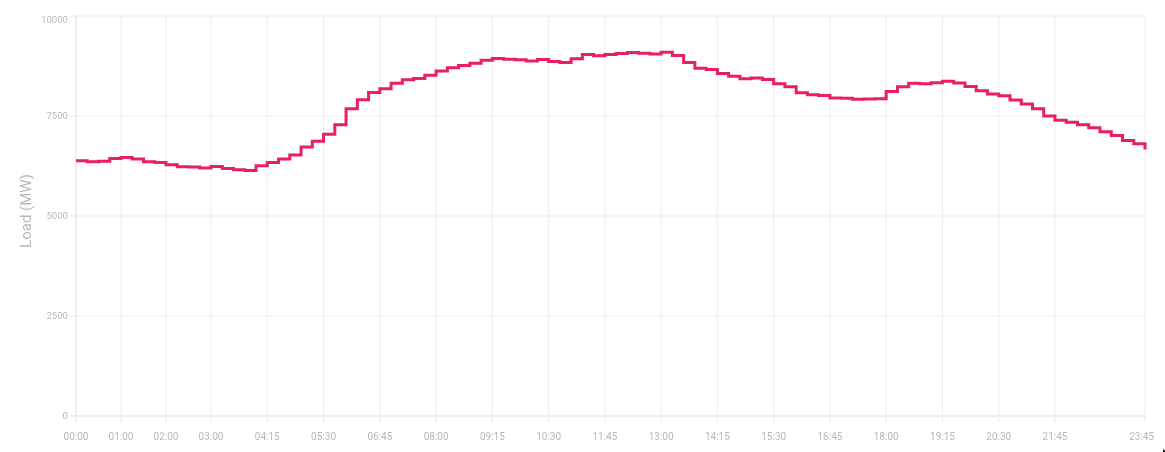
\includegraphics[width=1\linewidth]{images/load_figure.jpg}
    \caption{Zatížení soustavy 12.~03.~2026~\cite{entsoe}}
    \label{fig:load-example}
\end{figure}

Proti této poptávce stojí strana nabídky, kterou tvoří mix výrobních zdrojů~-- od solárních a~větrných parků přes jaderné elektrárny až po uhelné a~plynové bloky. Způsob, jakým výrobci svou energii na trhu nabízejí, jak se tyto zdroje za sebou řadí podle svých provozních nákladů a~jak z~tohoto mechanismu vzejde výsledná tržní cena, bude detailně rozebrán v~následující podkapitole.

\subsection{Strana nabídky a~princip Merit Order}
\label{subsec:merit-order}
Zatímco poptávka je dána spotřebou koncových spotřebitelů, stranu nabídky tvoří samotní výrobci elektřiny. Ti nabízejí svou dostupnou kapacitu na trhu, přičemž klíčovým mechanismem, který z~těchto nabídek utváří výslednou cenu, je takzvaný princip Merit Order (často překládaný jako závěrné pořadí zdrojů).

Merit Order je ekonomický model, který řadí dostupné výrobní zdroje na trhu vzestupně podle jejich krátkodobých mezních nákladů na výrobu jedné megawatthodiny (MWh) elektřiny~\cite{merit-order}. Mezní náklady představují pouze výdaje spojené se samotnou produkcí energie -- typicky se jedná o~cenu paliva a~u fosilních zdrojů také o~cenu emisních povolenek. Investiční náklady na původní výstavbu elektrárny se do tohoto mechanismu nezohledňují.

Podle tohoto pravidla se elektrárny do systému zapojují v~následujícím pořadí~\cite{merit-order}:
\begin{enumerate}
    \item \textbf{Obnovitelné zdroje energie (OZE)}: Solární, větrné a~průtočné vodní elektrárny mají mezní náklady blížící se nule, jelikož ke svému provozu nevyžadují nákup paliva. Na křivce nabídky tak figurují na prvním místě. 
    \item \textbf{Jaderné elektrárny:} Vyznačují se velmi nízkými variabilními palivovými náklady a~slouží jako stabilní základní zdroje
    \item \textbf{Uhelné elektrárny:} Jejich provozní náklady jsou určeny cenou uhlí a~nutností pokrýt emise nákupem povolenek. 
    \item \textbf{Plynové elektrárny:} Tyto zdroje mívají nejvyšší mezní náklady, dokážou však velice rychle startovat a~operativně pokrývat výkonové špičky. Často proto fungují jako takzvané špičkové zdroje na samém konci nabídkové křivky.
\end{enumerate}

Při určování tržní ceny burza postupně uspokojuje aktuální poptávku přijímáním nabídek od těch nejlevnějších zdrojů. Zdroj, jehož nabídka dorovná celkovou poptávku jako poslední, se stává tzv. závěrným zdrojem. Její nabídková cena se následně stává výslednou cenou na trhu pro daný časový interval. Tuto cenu obdrží všichni zapojení výrobci bez ohledu na to, jak nízké byly jejich vlastní mezní náklady~\cite{merit-order}.

\begin{figure}[htbp]
    \centering
    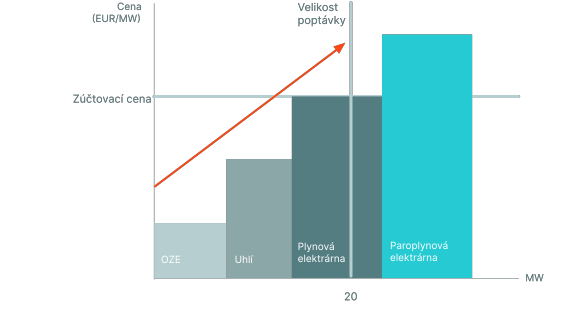
\includegraphics[width=1\linewidth]{images/graf-merit-order.png}
    \caption{Princip tvorby ceny pomocí Merit Order~\cite{merit-order}}
    \label{fig:merit-order}
\end{figure}

Z~tohoto mechanismu jasně vyplývá zásadní vliv počasí na volatilitu cen elektřiny. Pokud v~danou hodinu svítí slunce a~fouká vítr, trh je nasycen levnou energií z~obnovitelných zdrojů. Drahé fosilní zdroje tak vůbec nejsou k~pokrytí poptávky potřeba a~výsledná tržní cena výrazně klesá. Schopnost odhadnout výrobu z~obnovitelných zdrojů jsou proto pro úspěšnou predikci tržních cen naprosto stěžejní.

\subsection{Organizace denního trhu v~České republice}
V~České republice je organizátorem krátkodobého trhu s~elektřinou společnost OTE,~a.s. Stěžejní platformou pro obchodování je tzv. denní trh (DT)~\cite{ote-kratkodobe-trhy}, kde se nakupuje a~prodává elektrická energie s~dodávkou na následující den. Obchodování zde neprobíhá za jednu celodenní průměrnou cenu, nýbrž nezávisle pro dílčí časové úseky. Dlouhé roky tvořila základní obchodní periodu jedna hodina (výsledkem tedy bylo 24 cen denně). V~reakci na rostoucí podíl těžko predikovatelných obnovitelných zdrojů a~nutnost efektivnějšího vyrovnávání sítě však český trh od října 2025 přešel na 15minutové obchodní periody\footnote{Přechod na 15minutovou periodu proběhl dvoufázově: 1.~července 2024 pro zúčtování a~vnitrodenní trhy, a~následně 1.~října 2025 i~pro jednotný denní trh.}~\cite{ote-kratkodobe-trhy}. Každý den se tak nově skládá z~96 nezávislých obchodních intervalů\footnote{Případně 92 či 100 intervalů při přechodu na letní, respektive zimní čas.}, jejichž ceny jsou stanoveny v~eurech za megawatthodinu (EUR/MWh). Tento přechod radikálně zvýšil volatilitu na trhu a~znásobil nároky na automatizaci a~algoritmické řízení obchodních strategií.

Z~hlediska mechanismu funguje denní trh na principu uzavřené (slepé) aukce. Účastníci trhu (výrobci, dodavatelé či spekulativní obchodníci) zadávají do obchodního systému své nabídky a~poptávky ve formě cenových a~množstevních kroků. Všechny tyto individuální objednávky operátor trhu následně sloučí do souhrnné křivky nabídky (odrážející princip Merit Order) a~souhrnné křivky poptávky. Průsečík těchto dvou křivek pro každý z~96 denních intervalů určuje výslednou zúčtovací cenu a~celkové zobchodované množství.~\cite{ote-kratkodobe-trhy}\\

\begin{figure}[htbp]
    \centering
    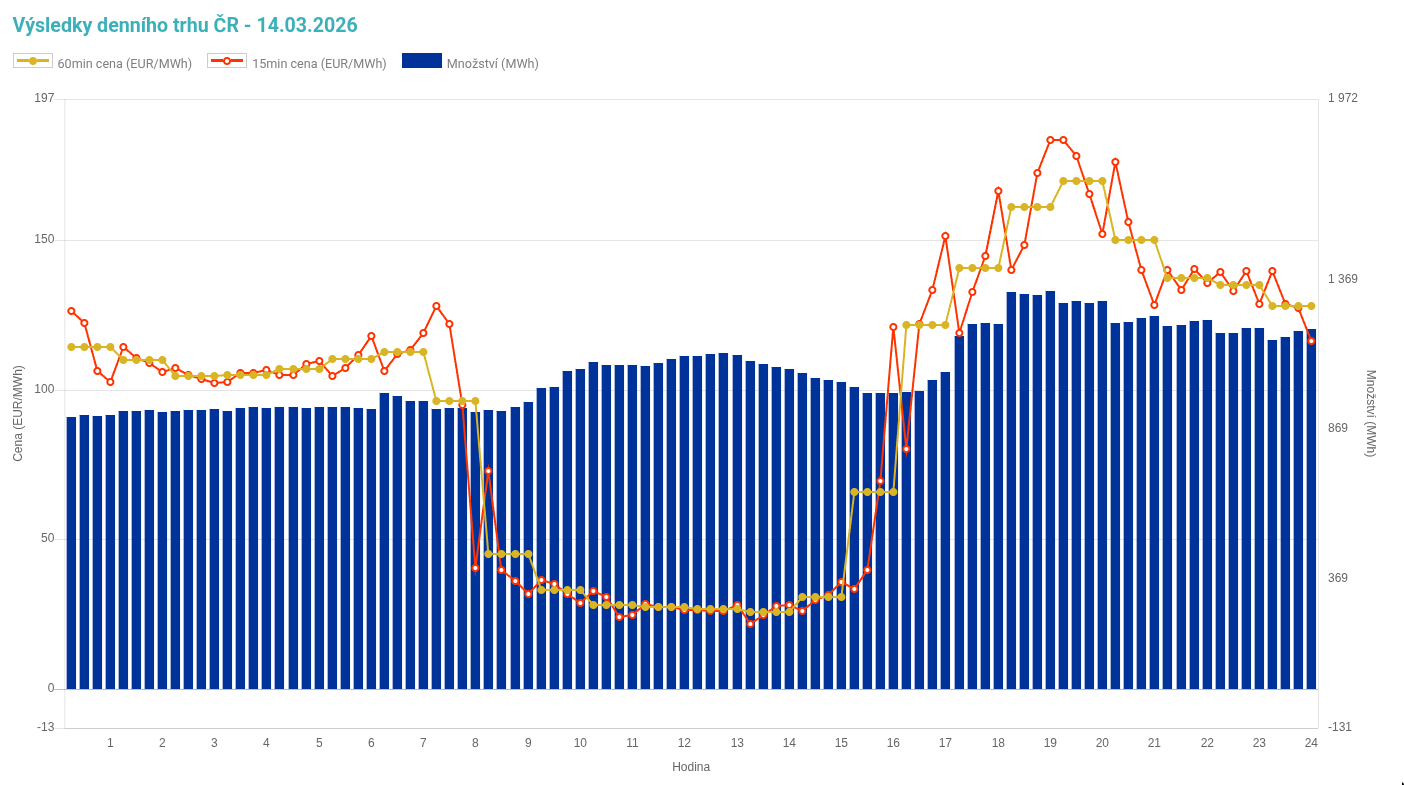
\includegraphics[width=1\linewidth]{images/ote-dt-vysledky.jpg}
    \caption{Výsledky denního trhu ČR -- 14.~3.~2026~\cite{ote-dt-vysledky}}
    \label{fig:dt-vysledky}
\end{figure}

Z~pohledu návrhu prediktivního modelu strojového učení je však zcela zásadní časový harmonogram celého procesu. Uzávěrka příjmu nabídek a~poptávek (tzv. Gate Closure Time) je pro celý zítřejší den striktně stanovena na 12:00 hodin dne předcházejícího dni dodávky (D-1)~\cite{ote-kratkodobe-trhy}. Krátce po poledni operátor trhu aukci vyhodnotí a~publikuje výsledné ceny pro všechny intervaly zítřejšího dne (viz Obrázek~\ref{fig:dt-vysledky}).



Tento časový milník představuje naprosto klíčové omezení pro vývoj jakéhokoliv prediktivního systému. Aby byl vytvořený model reálně využitelný v~praxi, musí vygenerovat kompletní predikci cen na zítřejší den (D) ještě před touto dvanáctou hodinou (v čase D-1).

Z~metodologického hlediska to znamená, že se model při tvorbě predikce nesmí opírat o~žádné informace, které v~reálném čase před dvanáctou hodinou nejsou známé. Může využívat pouze historické ceny do aktuálního okamžiku a~ranní předpovědi (např. očekávané zatížení soustavy od společnosti ENTSO-E) vydané pro zítřejší den. Důsledné dodržení této podmínky a~zamezení prosakování budoucích informací do trénovacích dat (tzv. data leakage) tvoří jeden z~hlavních pilířů této práce, čímž zajišťuje, že dosažené výsledky predikce jsou plně aplikovatelné v~reálném tržním prostředí.

\newpage
\section{Použité technologie}
Využití moderních softwarových nástrojů je nezbytným 
předpokladem pro úspěšnou realizaci jakéhokoliv data science projektu. 
Tato kapitola představuje technologický stack, který byl zvolen pro 
vývoj celého systému. Jelikož je projekt koncipován jako 
end-to-end řešení, použitý ekosystém musí pokrývat celý životní 
cyklus aplikace~-- od automatizovaného získávání a~předzpracování 
surových dat, přes trénování modelu strojového učení, až po finální 
nasazení a~vizualizaci výsledků v~rámci interaktivního webového rozhraní.

Celý systém byl vyvinut v~jazyce \textbf{Python}, který je dnes standardem v~oblasti umělé inteligence a~datové analytiky. Následující sekce představují klíčové knihovny a~frameworky využité v~jednotlivých fázích projektu.

\subsection{Jupyter Notebook}
Vývoj prediktivního systému není přímočarý proces, vyžaduje přístup spočívající v~neustálém testování hypotéz, ladění parametrů a~analýze dat. Pro tyto účely bylo využito interaktivní vývojové prostředí Jupyter Notebook, které se stalo standardem pro experimentální fáze projektů v~oblasti datové vědy a~strojového učení~\cite{jupyter}.

V~rámci tohoto projektu sloužil Jupyter Notebook jako primární nástroj pro experimentování s~různými architekturami modelů a~pro ladění jejich hyperparametrů. Interaktivní povaha prostředí umožnila okamžitou vizualizaci výsledků tréninku a~vyhodnocování predikčních metrik. Teprve ve chvíli, kdy byl kód v~notebooku dostatečně otestován a~model optimalizován, byly klíčové algoritmy přesunuty do produkčních Python skriptů pro integraci s~finální webovou aplikací.

\begin{figure}[htbp]
    \centering
    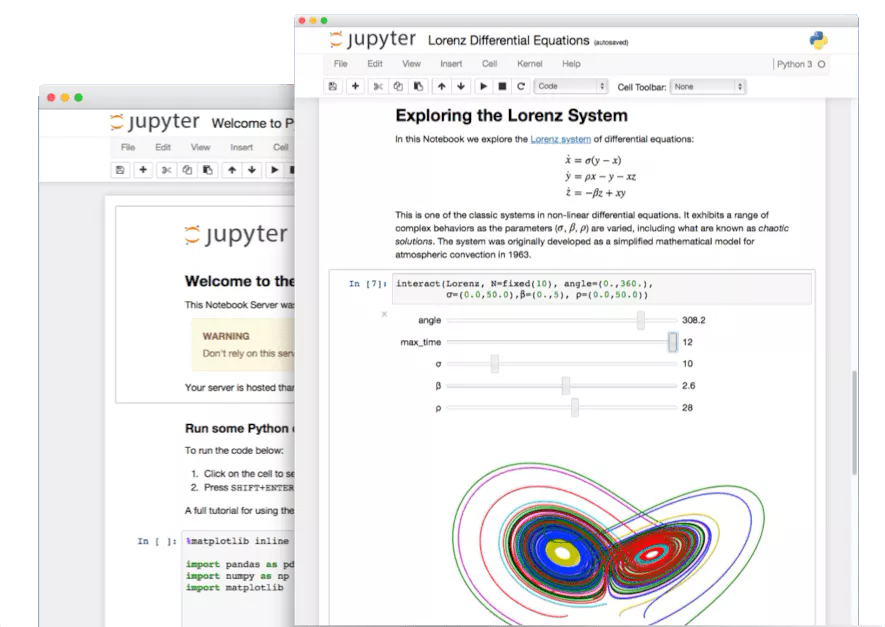
\includegraphics[width=0.9\linewidth]{images/jupyter-preview.png}
    \caption{Úkázka prostředí Jupyter Notebook~\cite{jupyter}}
    \label{fig:jupyter-preview}
\end{figure}
\subsection{Pandas}
Příprava kvalitního datasetu je často nejnáročnější fází celého projektu. Vzhledem k~tomu, že prediktivní systém zpracovává data z~více nezávislých zdrojů (budu rozebírat do detailu v~jiných kapitolách), bylo nutné zajistit jejich efektivní načítání, čištění, transformaci a~synchronizaci. K~tomuto účelu byla jako primární nástroj zvolena open-source knihovna Pandas~\cite{pandas-docs}.

Knihovna poskytuje vysoce výkonné a~snadno použitelné datové struktury, 
přičemž jejím stěžejním prvkem je objekt \textit{DataFrame}~\cite{pandas-dataframe}, jenž umožňuje 
pracovat s~daty ve formě dvourozměrných tabulek podobných relačním 
databázím. Pro projekt zabývající se predikcí cen na krátkodobých trzích 
s~elektřinou je Pandas naprosto nepostradatelný nástroj, neboť nabízí 
nativní a~vysoce optimalizovanou podporu pro práci s~časovými řadami. 

Díky pokročilým možnostem byla knihovna využita ke sjednocení časových kroků ze všech datových zdrojů, k~ošetření chybějících hodnot a~k~finálnímu spojení všech proměnných do jednoho uceleného trénovacího datasetu. 

\subsection{NumPy}
Zatímco Pandas slouží primárně pro manipulaci se strukturovanými daty a~časovými řadami, výpočetní jádro (backend) pro většinu těchto operací tvoří knihovna NumPy~\cite{numpy-docs}. Jedná se o~fundamentální balíček ekosystému Python pro vědecké a~numerické výpočty, který představuje průmyslový standard pro efektivní práci s~velkými objemy dat.

Hlavní síla knihovny spočívá v~implementaci výkonného vícerozměrného pole 
(\textit{ndarray}~\cite{numpy-ndarray}) a~široké škály matematických funkcí, 
jež nad těmito poli operují. V~porovnání se standardními datovými strukturami 
jazyka Python (jako jsou běžné seznamy, tzv. lists) dosahuje NumPy řádově 
vyšších rychlostí.

V~rámci realizovaného prediktivního systému funguje NumPy z~velké části na pozadí a~zajišťuje rychlé provádění transformací v~rámci objektů Pandas DataFrame. 

\subsection{Scikit-Learn}
Základním nástrojem pro implementaci algoritmů strojového učení v~rámci tohoto projektu se stala knihovna Scikit-Learn~\cite{scikit-learn}. Jedná se o~jeden z~nejrozšířenějších open-source nástrojů pro prediktivní analýzu dat v~ekosystému jazyka Python. Využití této knihovny v~této práci probíhalo ve dvou klíčových rovinách.

První z~nich se týkala nezbytné přípravy dat před samotným trénováním. Zásadním krokem v~každém projektu strojového učení je korektní rozdělení datasetu na trénovací a~testovací množinu. Jelikož cílem práce je predikce vývoje cen elektřiny v~čase, nebylo možné použít standardní náhodné rozdělení dat, které by vedlo k~závažnému úniku informací z~budoucnosti do trénovací fáze (tzv. data leakage). Pro tyto účely Scikit-Learn nabízí specializované nástroje, ty jsou v~detailu popsány v~pozdějších kapitolách.  

Druhou rovinou využití knihovny bylo vytvoření tzv. referenčního modelu. Pro tyto účely byla ze Scikit-Learn implementována lineární regrese (\textit{LinearRegression}~\cite{linear-regression}).

\subsection{XGBoost}
Zatímco knihovna Scikit-Learn poskytla základní infrastrukturu a~referenční modely, jako hlavní prediktivní engine celého systému byla zvolena knihovna XGBoost~\cite{xgboost} (eXtreme Gradient Boosting).V~současnosti patří XGBoost mezi nejpoužívanější a~nejvýkonnější algoritmy strojového učení pro práci se strukturovanými tabulkovými daty.

Z~technologického hlediska byla knihovna XGBoost do projektu začleněna především pro svou bezkonkurenční schopnost modelovat složité nelineární vztahy mezi velkým množstvím vstupních proměnných. Její implementace vyniká vysokou výpočetní efektivitou, vestavěnou podporou pro paralelní zpracování a~robustností vůči chybějícím či odlehlým hodnotám (outliers), které jsou pro energetické trhy typické. Detailní princip fungování tohoto algoritmu, bude rozebrán v~následujících kapitolách věnovaných samotné metodice modelování (viz Podkapitola \ref{subsubsec:xgboost}).

\subsection{Matplotlib}
Získání hlubšího vhledu do struktury dat a~srozumitelná prezentace dosažených výsledků jsou nepostradatelnou součástí každého analytického projektu. Pro tyto účely byla zvolena knihovna Matplotlib~\cite{matplotlib}, jež představuje absolutní základ a~průmyslový standard pro vizualizaci dat v~ekosystému jazyka Python.

Jedná se o~komplexní a~vysoce flexibilní nástroj pro tvorbu 2D grafů, který vývojáři poskytuje kontrolu nad každým grafickým elementem. 

\subsection{PostgreSQL}
Aby bylo možné prediktivní systém provozovat jako plnohodnotnou aplikaci (a nikoliv pouze jako lokální skript), bylo nutné zajistit robustní vrstvu pro ukládání dat. Pro tyto účely byl zvolen PostgreSQL~\cite{postgres}, pokročilý open-source relační databázový systém. V~současnosti se jedná o~jeden z~nejrespektovanějších standardů v~softwarovém inženýrství, který vyniká vysokou spolehlivostí, výkonem a~striktním dodržováním standardů jazyka SQL.

V~architektuře tohoto projektu plní PostgreSQL roli centrálního datového skladu. Slouží k~bezpečnému ukládání finálních predikcí vygenerovaných modelem a~také skutečných cen.

\newpage
\subsection{Flask}
Zatímco databáze a~modely strojového učení tvoří skryté jádro systému (tzv. backend), pro interakci s~okolním světem bylo potřeba vytvořit aplikační rozhraní. K~tomuto účelu byl nasazen Flask~\cite{flask}~-- odlehčený webový framework. Jeho hlavní předností je minimalistický přístup, vysoká flexibilita a~to, že vývojáři nevnucuje žádnou striktní strukturu projektu, což z~něj činí ideální nástroj pro rychlý vývoj. 

V~rámci celého systému funguje Flask jako hlavní spojovací článek. Aplikace ve Flasku naslouchá uživatelským požadavkům (HTTP requestům), na jejichž základě komunikuje s~databází PostgreSQL, odkud získává aktuální data. 

\subsection{APScheduler}
Pro zajištění plné autonomie prediktivního systému a~jeho přechod z~lokálního analytického skriptu v~produkční aplikaci bylo nezbytné implementovat mechanismus pro automatizované spouštění úloh na pozadí. K~tomuto účelu byla využita knihovna APScheduler~\cite{apscheduler} (Advanced Python Scheduler). Jedná se o~lehký, ale vysoce flexibilní nástroj pro plánování úloh přímo uvnitř běžících Python aplikací, který nabízí funkcionalitu srovnatelnou se systémovými \textit{cron} démony, avšak s~výhodou přímé integrace do aplikačního kódu a~paměťového prostoru.

Nasazení tohoto plánovače si vyžádala samotná povaha denního trhu s~elektřinou, který operuje podle striktního časového harmonogramu. V~rámci architektury aplikace plní APScheduler roli hlavního orchestrátoru a~zajišťuje pravidelné spouštění kritických procesů bez nutnosti jakéhokoliv manuálního zásahu.

\subsection{Docker}
Zásadním problémem při vývoji komplexních softwarových systémů, obzvláště těch, které kombinují databáze, modely strojového učení a~webové servery, je zajištění jejich bezproblémové přenositelnosti mezi různými výpočetními prostředími. K~eliminaci známého problému „na mém počítači to funguje“ byla do projektu implementována platforma Docker~\cite{docker}, jež představuje současný standard v~oblasti kontejnerizace aplikací.

Docker umožňuje zabalit celou aplikaci včetně všech jejích závislostí, knihoven a~konfiguračních souborů do izolovaného softwarového kontejneru. V~rámci tohoto projektu byla kontejnerizace využita k~oddělení hlavních komponent systému~-- webového serveru (Flask s~integrovaným modelem a~plánovačem APScheduler) a~databázového serveru (PostgreSQL). Pomocí nástroje \textit{Docker Compose}~\cite{docker-compose} je následně možné celou tuto multi-kontejnerovou architekturu definovat jediným konfiguračním souborem a~spustit ji na libovolném serveru či operačním systému jediným příkazem. Tento přístup nejenže radikálně zjednodušuje případné nasazení (deployment) aplikace do produkčního cloudového prostředí, ale také garantuje absolutní reprodukovatelnost celého vývojového prostředí.

\newpage
\subsection{Technologie uživatelského rozhraní}
Přestože je projekt primárně datovou a~backendovou aplikací, disponuje plnohodnotným uživatelským rozhraním. Architektura frontendu byla navržena s~maximálním ohledem na jednoduchost a~výkon~-- s~cílem vyhnout se zbytečné složitosti padla volba na sadu minimalistických, avšak vysoce efektivních nástrojů.

O~vizuální stránku aplikace se stará \textbf{Tailwind CSS}~\cite{tailwind}. Jedná se o~populární framework, který umožňuje stylovat uživatelské rozhraní extrémně rychle přímo v~HTML šablonách pomocí předpřipravených tříd, čímž odpadá nutnost psát a~udržovat rozsáhlé externí kaskádové styly.
\begin{lstlisting}[style=htmlstyle, caption={Příklad použití Tailwind CSS}]
<div>
    <div class="text-xl font-medium text-black dark:text-white">
        ChitChat
    </div>
    <p class="text-gray-500 dark:text-gray-400">
        You have a~new message!
    </p>
</div>
\end{lstlisting}


Pro zajištění dynamického chování webu bez nutnosti psaní složitého asynchronního JavaScriptu (AJAX) byla využita knihovna \textbf{HTMX}~\cite{htmx}. Tato minimalistická technologie umožňuje odesílat požadavky na server a~plynule aktualizovat pouze specifické části webové stránky přímo pomocí HTML atributů.
\begin{lstlisting}[style=htmlstyle, caption={Příklad použití HTMX}]
<button 
    hx-post="/clicked"
    hx-trigger="click"
    hx-target="#parent-div"
    hx-swap="outerHTML">
    Click Me!
</button>
\end{lstlisting}
Toto lze přeložit jako:
Když uživatel klikne na toto tlačítko, odešlete HTTP POST požadavek na „/clicked“ a~pomocí obsahu z~odpovědi nahraďte v~DOMu element s~ID „parent-div“.

Finální prezentaci dat v~prohlížeči následně doplňuje knihovna \\ \textbf{Google Charts}~\cite{google-charts}. Zatímco backendový Matplotlib sloužil primárně k~nalýze a~evaluaci během vývoje, Google Charts byly nasazeny na klientské straně pro interaktivní a~vizuálně atraktivní vykreslování cenových křivek, které uživateli umožňují plynule zkoumat detaily predikovaných a~skutečných hodnot napříč časem.

\newpage
\section{Datové zdroje a~výběr vstupních příznaků}
Jak bylo detailně popsáno v~teoretické části práce, cena elektřiny na krátkodobém denním trhu nepodléhá náhodě. Její hodnota se formuje prostřednictvím průniku křivek nabídky a~poptávky, a~to v~přísném souladu s~efektem závěrného pořadí zdrojů (Merit Order). Hluboké pochopení těchto tržních mechanismů je pro návrh prediktivního systému naprosto klíčové, neboť umožňuje cíleně identifikovat a~vybrat takové vstupní parametry (features), které fundamentálně ovlivňují chování trhu.

Pro účely trénování a~evaluace modelu bylo jako optimální časové okno zvoleno souvislé období kalendářních let 2023, 2024 a~2025. Aktuální rok 2026 nebyl do hlavní trénovací datové sady plně zahrnut z~důvodu své nekompletnosti k~datu zpracování práce. Naopak starší data, zejména z~kritického roku 2022, byla z~datasetu záměrně vyloučena. Rok 2022 se totiž vyznačoval extrémní cenovou volatilitou, nestandardním chováním trhu a~šoky způsobenými eskalací geopolitické situace a~následnou energetickou krizí v~Evropě. Zahrnutí těchto vysoce anomálních dat by s~vysokou pravděpodobností degradovalo schopnost algoritmu generalizovat a~správně identifikovat běžné sezónní a~denní vzorce za standardních tržních podmínek.

Následující kapitoly detailně mapují celý proces budování trénovacího datasetu. Nejprve budou představeny primární zdroje, z~nichž byla nezbytná data získávána. Následně je rozebrán význam jednotlivých zvolených prediktorů v~kontextu energetiky~-- od vlivu obnovitelných zdrojů až po plánované zatížení sítě. Závěr kapitoly se pak věnuje nezbytnému předzpracování surových dat, ošetření anomálií a~tvorbě odvozených proměnných, jež předcházely samotnému trénování algoritmu.

\subsection{Operátor trhu s~elektřinou (OTE)}
Česká společnost OTE,~a.s. funguje jako centrální organizátor krátkodobého trhu s~elektřinou a~plynem. Její veřejné rozhraní tak důležitý, a~především zcela legitimní zdroj dat pro tuto práci. Z~technického hlediska bylo získávání historických dat realizováno formou hromadného stahování ucelených ročních zpráv~\cite{ote-rocni-zprava} (ročních datových reportů), což zajistilo maximální konzistenci a~celistvost potřebné historie bez výpadků. Z~těchto ročních souborů byly následně extrahovány klíčové cenové informace, které tvoří jak samotnou cílovou proměnnou modelu, tak zásadní historické prediktory.

Z~technologického hlediska poskytuje OTE svá historická data primárně 
ve formátu tabulek pro tabulkové procesory (MS Excel s~příponou \texttt{.xlsx}). Ačkoliv knihovna Pandas disponuje nástroji pro přímé čtení těchto formátů, OTE do roční zprávy uvádí příliš mnoho údajů, které v~datasetu nepotřebujeme. Z~důvodu optimalizace 
datové pipeline a~sjednocení formátů byly zdrojové roční zprávy 
nejprve manuálně konvertovány do čistého textového formátu CSV . Tento mezikrok zajistil řádově rychlejší načítání dat do operační paměti a~eliminoval problémy se skrytým formátováním buněk v~Excelu. \\

\begin{lstlisting}[language=Python, caption={Načtení transformovaných dat OTE do knihovny Pandas}]
import pandas as pd

df = pd.read_csv("../data/ote_2022-12-25_2025-12-31_gas_prices.csv", sep=";")

cols_to_convert = [
    "Vazeny prumer cen (EUR/MWh)",
]

for col in cols_to_convert:
    if df[col].dtype == object:
        df[col] = df[col].astype(str).str.replace(",", "")
    df[col] = pd.to_numeric(df[col], errors="coerce")
    
df["Plynarensky den"] = pd.to_datetime(df["Plynarensky den"], dayfirst=True)

clean_df = df[["Plynarensky den", "Vazeny prumer cen (EUR/MWh)"]].rename(columns={
    "Plynarensky den": "date",
    "Vazeny prumer cen (EUR/MWh)": "gas_price"
})

clean_df.to_csv("../data/ote_gas_prices.csv", sep=";", index=False)
\end{lstlisting}

Tento systematický přístup~-- tedy stažení původní roční zprávy ve formátu Excelu, její bezprostřední konverze do textového souboru CSV a~následné načtení pomocí optimalizované funkce \texttt{read\_csv()} z~knihovny Pandas~-- byl striktně uplatněn plošně. Obdobným způsobem tak bylo postupováno při extrakci veškerých dalších historických dat z~rozhraní operátora trhu. Tímto jednotným postupem byla zajištěna maximální konzistence a~stabilita celého procesu datové přípravy.

\subsubsection{Ceny elektrické energie na denním trhu}
Základním datovým bodem stahovaným z~rozhraní OTE byly zúčtovací ceny elektřiny. Jak již bylo zmíněno v~teoretické části, od 1.~října 2025 přešel denní trh na 15minutové obchodní periody. Jelikož trénovací dataset pokrývá i~roky 2023 a~2024, kdy trh operoval na hodinové bázi, bylo nutné starší historická data příslušně transformovat na 15minutové rozlišení\footnote{Tato nutnost transformace se vztahuje i~na období od počátku roku 2025 do 30. září}. Tento nezbytný krok převzorkování (resampling) je po technické stránce detailně popsán v~závěrečné podkapitole věnované předzpracování dat (viz Podkapitola \ref{subsec:transformace-hodinovych-period}).

Tyto hodnoty v~první řadě slouží jako \textit{labels} (cílové hodnoty) pro 
trénování algoritmu a~následné ověření jeho přesnosti. Současně však byly 
historické ceny využity jako silné vstupní příznaky (features). Modelu je vždy 
předložena cena elektřiny v~identickém 15minutovém okně přesně před týdnem 
($t-7$ dní). Tento parametr (tzv. lag) pomáhá algoritmu zachytit silnou 
týdenní sezónnost trhu~-- například fakt, že víkendové dny mají z~důvodu nižší 
průmyslové aktivity odlišný cenový profil než dny pracovní.

\subsubsection{Agregované cenové profily trhu}
\label{subsubsec:agregovane-cenove-profily-trhu}
Samotná 15minutová data z~denního trhu vykazují značnou volatilitu a~jsou zatížena krátkodobým šumem. V~energetické praxi se proto pro celkové zhodnocení cenové hladiny využívají standardizované burzovní indexy, které rozdělují den podle typického chování spotřebitelů a~průmyslu. Aby model získal tento širší kontext o~charakteru daného dne, byly ze surových dat odvozeny tři klíčové parametry:

\begin{itemize}
    \item \textbf{Základní zatížení (Base Load):} Představuje celodenní průměrnou cenu napříč všemi obchodními intervaly. Slouží jako indikátor obecné cenové hladiny (zda je na trhu energie celkově 
    levná, nebo drahá).
    
    \item \textbf{Špičkové zatížení (Peak Load):} Průměrná cena v~době nejvyšší energetické poptávky, jež je tradičně definována v~čase od 8:00 do 20:00. V~této době běží většina průmyslových podniků, síť je nejvíce zatížena a~ceny logicky dosahují denních maxim.
    
    \item \textbf{Mimošpičkové zatížení (Off-peak Load):} Průměrná cena v~nočních hodinách\footnote{Časové bloky od 00:00 do 8:00 a~následně od 20:00 do 24:00.}. V~tomto období spotřeba radikálně klesá, drahé zdroje se odpojují a~na trhu zůstává levnější energie.
\end{itemize}

Díky těmto agregovaným profilům je prediktivní algoritmus schopen lépe vnímat celodenní trend a~není závislý pouze na izolovaných 15minutových výkyvech.

Je důležité podotknout, že tento koncept rozdělení dne na bloky Base, Peak a~Off-peak se v~rámci tvorby datasetu ukázal jako natolik robustní, že byl následně aplikován nejen na ceny elektřiny, ale stejnou logikou i~na další nezávislé proměnné. V~následujících kapitolách tak bude tento přístup využit například pro agregaci očekávané výroby z~obnovitelných zdrojů (slunce a~vítr), kde model díky tomu získá informaci, zda bude vysoká produkce solární energie korelovat s~obdobím nejvyšší průmyslové poptávky. 

\newpage
\begin{lstlisting}[language=Python, caption={Výpočet Base load, Peak load a~Off-peak load}]
raw_hour = df["time_interval"].str.split(":").str[0]
df["hour"] = raw_hour.str.replace(r"\D", "", regex=True).astype(int)

is_peak_hours = (df["hour"] >= 8) & (df["hour"] < 20)
df["Market Period"] = "Off-peak"
df.loc[is_peak_hours, "Market Period"] = "Peak"

df["day"] = pd.to_datetime(df["day"])

daily_results = []

for current_date, group in df.groupby("day"):
    peak_group = group[group["Market Period"] == "Peak"]
    offpeak_group = group[group["Market Period"] == "Off-peak"]
    
    base_price = group["price"].mean()
    peak_price = peak_group["price"].mean() if not peak_group.empty else np.nan
    offpeak_price = offpeak_group["price"].mean() if not offpeak_group.empty else np.nan
    
    daily_results.append({
        "Date": current_date.strftime("%Y-%m-%d"),
        "Baseload Price": round(base_price, 2) if pd.notna(base_price) else "",
        "Peakload Price": round(peak_price, 2) if pd.notna(peak_price) else "",
        "Off-peak Price": round(offpeak_price, 2) if pd.notna(offpeak_price) else ""
    })
\end{lstlisting}

\subsubsection{Ceny zemního plynu}
Velmi specifickým, avšak kriticky důležitým parametrem získaným z~rozhraní OTE, je cena zemního plynu na vnitrodenním trhu (viz roční zpráva, komodita plyn~\cite{ote-rocni-zprava}). Jak bylo definováno v~teoretické části (viz efekt závěrného pořadí zdrojů, podkapitala \ref{subsec:merit-order}), plynové elektrárny často figurují jako poslední, nejdražší zapínané zdroje pro pokrytí špičkové poptávky. Cena plynu se tak stává marginální cenou, která přímo diktuje finální cenu elektřiny pro celý trh. Do modelu byla vstupována jak aktuální cena plynu pro daný den, tak její hodnota zpožděná o~jeden týden ($t - 7$). Tento fundamentální parametr umožňuje modelu elegantně pochopit náhlé skoky v~cenách elektřiny, které by ze samotných historických řad elektřiny nebyly odvoditelné.

\newpage
\subsection{Informační platforma SMARD.de}
Český trh s~elektřinou nefunguje izolovaně. Naopak je prostřednictvím přeshraničních kapacit silně provázán s~okolními státy, především pak s~německou obchodní zónou. Vzhledem k~obrovskému instalovanému výkonu německých obnovitelných zdrojů diktuje tamní výroba a~spotřeba často cenový trend pro celý středoevropský region. Z~tohoto důvodu byla pro tvorbu trénovacího datasetu využita datová 
platforma SMARD.de~\cite{smard-de}, provozovaná německým Spolkovým úřadem pro sítě (Bundesnetzagentur), z~níž byly extrahovány klíčové fundamentální parametry o~stavu německé soustavy.

Na rozdíl od českého operátora trhu umožňuje německá platforma SMARD.de exportovat definované časové řady přímo v~nativním a~strojově vysoce přívětivém formátu CSV. Datové sady obsahující německou generaci z~OZE a~celkové zatížení soustavy tak mohly být do analytického prostředí ingestovány bez nutnosti předchozí manuální konverze. Rozhraní Pandas dokáže tyto soubory zpracovat velmi efektivně, což umožnilo okamžitou aplikaci agregačních funkcí pro výpočet denních profilů (Base, Peak a~Off-peak load).

\subsubsection{Výroba z~obnovitelných zdrojů (Vítr a~Slunce)}
Produkce solárních a~větrných elektráren má díky svým téměř nulovým mezním nákladům největší vliv na stlačování ceny elektřiny směrem dolů. Pro trénování modelu byly ze systému získány dva typy vstupů: historické předpovědi výroby na následující den (day-ahead forecast) a~reálná skutečná výroba zpožděná o~jeden týden ($t-7$).

Při zpracování těchto časových řad bylo nutné zohlednit technologické omezení spojené s~nasazením modelu do produkčního prostředí. Ačkoliv pro historická trénovací data lze z~platformy SMARD.de dohledat předpovědi v~plném 15minutovém rozlišení, v~čase reálné predikce se nepodařilo zajistit bezplatný datový zdroj, který by takto granulární předpovědi na následující den spolehlivě poskytoval.

Aby byla zachována striktní konzistence mezi daty použitými pro učení modelu a~daty vstupujícími do reálné produkční predikce, byl tento rozpor vyřešen záměrnou agregací dostupných historických řad do ucelených denních profilů. Na proměnné byl aplikován totožný přístup jako u~cen z~OTE (viz podkapitola~\ref{subsubsec:agregovane-cenove-profily-trhu}) a~pro každý den byl vypočítán průměrný očekávaný \textit{Base Load}, \textit{Peak Load} a~\textit{Off-peak Load} solární a~větrné generace. Model tak nedisponuje informací o~přesném 15minutovém výkyvu počasí, ale má k~dispozici robustní znalost o~celkovém denním trendu. Alternativní zdroj, ze kterého prediktivní systém stahuje tyto agregované hodnoty v~reálném čase, je detailně popsán v~příslušné kapitole (viz Podkapitola \ref{subsec:spot-renewables}).

Je vhodné na tomto místě explicitně zdůraznit, že do prediktivního modelu nebyla záměrně vůbec zahrnuta data o~očekávané výrobě ze solárních a~větrných elektráren na území České republiky. Ačkoliv je cílem algoritmu predikovat tuzemské ceny, instalovaný výkon české fotovoltaiky a~obzvláště větrné energetiky je v~porovnání se sousedním Německem řádově nižší. V~rámci propojeného evropského trhu má tak lokální česká výroba z~těchto zdrojů na finální formování ceny pouze marginální vliv, který je zcela pohlcen masivními objemy levné energie proudící z~německé soustavy. Vyřazení těchto redundantních proměnných navíc přispělo ke snížení komplexity modelu a~ochraně algoritmu před zbytečným informačním šumem.

\subsubsection{Zatížení něměcké soustavy}
Do datasetu byly jako zásadní prediktory zařazeny jak předpovědi zatížení na následující den (day-ahead forecast), tak i~skutečné hodnoty zatížení ve stejném 15minutovém intervalu předchozího týdne ($t-7$). Kombinace těchto dvou příznaků dává modelu jasnou informaci o~celkovém tlaku na energetickou síť v~daném čase.

\subsubsection{Ostatní zdroje výroby v~Německu (Experimentální příznaky)}
\label{subsubsec:ostatni-zdroje-vyroby-nemecko}
Poslední skupinou dat získanou ze SMARD.de byla reálná 15minutová výroba z~konvenčních a~ostatních zdrojů (např. černouhelné a~hnědouhelné elektrárny, biomasa či přečerpávací vodní elektrárny). Tyto hodnoty byly do modelu vloženy ve formě zpožděných příznaků z~minulého týdne ($t-7$).

Zařazení takto granulárních informací o~jednotlivých energetických mixech bylo koncipováno jako experimentální část feature engineeringu. Cílem je zjistit, zda například informace o~historickém spínání německých přečerpávacích elektráren nese pro predikci české ceny nějakou skrytou, strojovým učením detekovatelnou hodnotu. Skutečná prediktivní síla a~relevance těchto konkrétních parametrů bude exaktně vyhodnocena v~pozdějších fázích projektu pomocí analýzy důležitosti příznaků . Pokud se prokáží jako redundantní či obsahující pouze šum, budou z~konečného datasetu odstraněny.

\subsection{ENTSO-E Transparency Platform}

Zatímco německá data poskytla modelu nezbytný kontext o~masivní výrobě z~obnovitelných zdrojů, pro přesnou predikci lokální ceny bylo nutné integrovat detailní informace o~stavu domácí sítě. K~tomuto účelu byla využita platforma Transparency Platform, kterou provozuje Evropská síť provozovatelů přenosových soustav pro elektřinu (ENTSO-E)~\cite{entsoe}. Tento systém funguje jako centrální a~standardizovaný repozitář fundamentálních dat pro všechny evropské energetické trhy.

Pro automatizované získávání dat z~této platformy je vyžadována oficiální registrace a~schválení žádosti o~přidělení bezpečnostního API klíče. Využití oficiálního REST API rozhraní~\cite{entsoe-api} nebylo v~rámci tohoto projektu omezeno pouze na jednorázové stažení historického datasetu pro natrénování modelu. Toto API tvoří kritickou datovou infrastrukturu celé aplikace. Plánovač úloh (APScheduler) jej využívá ke stahování těch absolutně nejaktuálnějších hodnot těsně před každým spuštěním denní predikce.

Integrace dat z~evropské platformy ENTSO-E představovala po softwarové stránce nejkomplexnější část procesu sběru. Oficiální REST API vyžaduje autentizaci pomocí bezpečnostního tokenu a~parametry dotazu (jako je definice obchodní zóny, typ dokumentu a~časové okno) se předávají primárně přes URL parametry.

\newpage
Kritickým specifikem tohoto rozhraní je striktní požadavek na formátování času. Veškeré časové značky ohraničující dotazované období \\ (parametry \texttt{periodStart} a~\texttt{periodEnd})~\cite{entsoe-api} musí být na server odesílány výhradně v~koordinovaném světovém čase (UTC). Vzhledem k~tomu, že český energetický trh operuje v~lokálním středoevropském čase (CET), respektive v~letním čase (CEST), vyžadovalo to na straně aplikace implementovat pečlivou konverzi časových zón před každým odesláním požadavku. Tímto krokem bylo striktně zamezeno jakýmkoliv fázovým posunům a~chybnému spárování dat.

\begin{lstlisting}[language=Python, caption={Funkce na převod CET/CEST na UTC}]
def convert_local_midnight_to_utc(date_str):
    pure_date = datetime.strptime(date_str, "%Y-%m-%d").date()
    prague_tz = ZoneInfo("Europe/Prague")
    local_midnight = datetime.combine(pure_date, time.min, tzinfo=prague_tz)
    utc_dt = local_midnight.astimezone(ZoneInfo("UTC"))
    
    # ENTSO-E vyzaduje format YYYYMMDDHHmm
    return utc_dt.strftime("%Y%m%d%H%M")
\end{lstlisting}

Dalším významným technologickým omezením samotného API je maximální povolená délka dotazovaného období. Systém provozovatele z~důvodu ochrany proti přetížení neumožňuje stáhnout data za období delší než jeden rok v~rámci jediného HTTP požadavku. Při získávání obsáhlých historických datasetů pokrývajících více let tak bylo nutné implementovat iterativní stahování, které celkový časový úsek automaticky rozdělilo na menší, maximálně roční intervaly.

Zásadním specifikem tohoto rozhraní je fakt, že serverové odpovědi nejsou vraceny v~dnes standardním formátu JSON, nýbrž ve striktně strukturovaném značkovacím jazyce XML (eXtensible Markup Language). Pro extrakci samotných číselných hodnot předpovědí a~skutečného zatížení tak bylo nezbytné implementovat v~jazyce Python specializovanou logiku pro průchod uzly XML stromu. 

Pro samotnou síťovou komunikaci a~odesílání HTTP požadavků na API rozhraní byla napříč celým projektem zvolena široce využívaná externí knihovna \texttt{requests}~\cite{python-requests}. Z~bezpečnostních důvodů není autentizační token předáván otevřeně v~URL adrese, ale je injektován přímo do hlavičky HTTP požadavku (Headers). Následné zpracování XML dokumentu vyžaduje aplikaci knihovny \texttt{xml.etree.ElementTree}~\cite{xml-parser} a~především korektní definici jmenných prostorů (XML namespaces), pod kterými jsou jednotlivé datové bloky (období a~měřené body) uloženy.

\newpage
\begin{lstlisting}[language=Python, caption={Implementace dotazu na ENTSO-E API a~hierarchické parsování XML odpovědi}]
hourly_data = []

def parse_xml_response(data, xml_text, namespace):
    root = ET.fromstring(xml_text)
    ns = {"ns": namespace}
    
    for period_block in root.findall(".//ns:Period", ns):
        day = period_block.find("ns:timeInterval/ns:start", ns).text
        
        for point in period_block.findall("ns:Point", ns):
            quantity = float(point.find("ns:quantity", ns).text)
            
            data.append(quantity)

headers = {
  "SECURITY_TOKEN": API_KEY 
}

url = "https://web-api.tp.entsoe.eu/api"
params = {
    'documentType': 'A65',
    'processType': 'A16',
    'outBiddingZone_Domain': '10YCZ-CEPS-----N',
    'periodStart': convert_local_midnight_to_utc('2022-12-25'),
    'periodEnd': convert_local_midnight_to_utc('2023-01-01'),
}

response = requests.get(url, params=params, headers=headers)

parse_xml_response(hourly_data, response.text, "urn:iec62325.351:tc57wg16:451-6:generationloaddocument:3:0")
\end{lstlisting}

\subsubsection{Zatížení české soustavy}
Nejdůležitějším domácím fundamentem je bezesporu celková poptávka po elektrické energii. Z~platformy ENTSO-E byly pro území České republiky extrahovány dvě klíčové proměnné v~15minutovém rozlišení. První z~nich je oficiální předpověď zatížení sítě na následující den (day-ahead load forecast), kterou vydává provozovatel přenosové soustavy (ČEPS)~\cite{ceps}. Druhou proměnnou je reálné, skutečně naměřené zatížení sítě zpožděné přesně o~jeden týden ($t-7$).

Tato kombinace poskytuje modelu extrémně silný prediktivní signál. Model díky předpovědi ví, jaká bude očekávaná celková spotřeba (např. vlivem ranní špičky nebo mrazivého počasí), a~zároveň díky týdennímu lagu ($t-7$) dokáže korigovat systematické odchylky a~vnímat přirozený cyklus pracovních dnů a~víkendů v~českém průmyslu.

\subsubsection{Ostatní zdroje výroby v~ČR (Experimentální příznaky)}
Identicky jako pro něměcký trh (viz Podkapitola~\ref{subsubsec:ostatni-zdroje-vyroby-nemecko}) byla z~ENTSO-E stažena i~historická data o~fyzické výrobě z~jednotlivých zdrojů na území ČR (např. jaderné, uhelné a~plynové elektrárny, přečerpávací vodní zdroje). Do trénovacího datasetu byly tyto hodnoty vloženy v~podobě zpožděných příznaků z~minulého týdne ($t-7$).

Také v~tomto případě se jedná o~experimentální rozšíření sady příznaků (feature engineering). Záměrem je otestovat hypotézu, zda specifické vzorce chování domácích konvenčních zdrojů (například historické spínání drahých plynových turbín v~časech špičky) nenesou dodatečnou informaci pro upřesnění cenové predikce. Nakolik jsou tyto lokální produkční proměnné pro model skutečně přínosné, případně zda je jejich vliv zcela zastíněn dominantními německými OZE a~celkovým zatížením sítě, bude následně exaktně prokázáno v~rámci vyhodnocení důležitosti příznaků. 

\subsection{Ceny emisních povolenek (oEnergetice.cz)}
Posledním, avšak z~hlediska cenotvorby naprosto fundamentálním prediktorem zahrnutým do trénovacího datasetu, je cena evropských emisních povolenek (EUA). Jak vyplývá z~principu závěrného pořadí zdrojů (Merit Order), jsou to velmi často právě fosilní elektrárny (uhelné a~plynové), které pokrývají špičkovou poptávku a~určují finální cenu na trhu. Jelikož jsou tito producenti povinni nakupovat emisní povolenky za každou vypuštěnou tunu CO$_2$, promítá se hodnota tohoto instrumentu přímo do jejich variabilních nákladů, a~potažmo do velkoobchodní ceny elektrické energie.

Historická data o~vývoji cen emisních povolenek byla získána z~odborného energetického portálu oEnergetice.cz~\cite{oenergetice}. Z~metodického hlediska je vhodné uvést, že se jednalo o~jediný datový zdroj v~rámci celého projektu, k~jehož strojovému vytěžení bylo nezbytné využít placené služby. Ačkoliv jsou historické průběhy cen na daném portálu veřejně vizualizovány formou interaktivních grafů, odkud by je bylo možné s~vynaložením extrémního úsilí manuálně odečítat, pro získání ucelené a~přesné časové řady v~machine-readable formátu (strojově čitelný export) bylo využito prémiového předplatného. Tento krok zajistil maximální přesnost vstupních dat bez rizika lidského pochybení při manuálním přepisu. Získané denní zavírací ceny (close prices) emisních povolenek byly následně do trénovací matice distribuovány jako konstantní hodnota pro všechny 15minutové intervaly příslušného obchodního dne.

Získané denní zavírací ceny (close prices) emisních povolenek byly následně do trénovací matice distribuovány jako konstantní hodnota pro všechny 15minutové intervaly příslušného dne. Specifikem tohoto finančního instrumentu je však skutečnost, že se s~ním na burze obchoduje výhradně v~rámci standardních pracovních dnů. Ve staženém datasetu tak přirozeně chyběly záznamy pro víkendy a~státní svátky. Pro zachování striktní kontinuity časové řady a~zamezení vzniku prázdných hodnot (tzv. NaN) byl tento datový výpadek vyřešen metodou \textit{forward-fill}. Hodnota povolenky z~posledního známého obchodního dne (typicky páteční zavírací cena) tak byla automaticky zkopírována i~do všech intervalů bezprostředně následujících neobchodních dnů, dokud nedošlo k~novému stanovení ceny při otevření trhu.

\newpage
\section{Předzpracování dat a~sestavení datasetu}
Surová data představují nezbytný základ pro trénování modelu, avšak ve svém původním stavu nejsou pro algoritmy strojového učení přímo použitelná. Reálné časové řady z~energetických trhů jsou typicky zatíženy řadou nedokonalostí~-- od různé vzorkovací frekvence napříč různými roky, přes chybějící záznamy (tzv. NaN hodnoty), až po nutnost vzájemného propojení zcela oddělených datových zdrojů.

Tato kapitola detailně popisuje proces čištění, transformace a~finálního sestavení datasetu. Cílem této fáze je sjednotit všechny nezávislé vstupy do jednoho spojitého celku a~vytvořit takové odvozené proměnné, které algoritmu maximálně usnadní detekci skrytých nelineárních závislostí.

\subsection{Transformace hodinových period}
\label{subsec:transformace-hodinovych-period}
Základním technickým předpokladem pro spojení dat z~více nezávislých zdrojů (tzv. data merge) je existence identické a~plně spojité časové osy. Cílem prediktivního systému bylo dodávat výstupy v~15minutovém rozlišení. Zatímco některá zahraniční data (např. z~německého trhu přes SMARD) byla k~dispozici v~tomto detailním formátu, historická data z~českého prostředí~-- a~to jak zúčtovací ceny z~operátora OTE, tak i~vybrané české časové řady ze systému ENTSO-E~-- operovala primárně na hodinové bázi. Pro sjednocení všech množin tak bylo nezbytné provést umělé zvýšení vzorkovací frekvence těchto hodinových datasetů.

Jelikož zúčtovací cena (v~EUR/MWh) či průměrné hodinové zatížení představují konstantní hodnotu platnou pro celý 60minutový blok, nebylo by fyzikálně ani ekonomicky smysluplné aplikovat jakoukoliv formu matematické interpolace. Každá původní hodina musela být exaktně rozdělena na čtyři identické 15minutové úseky se stejnou hodnotou.

Tento proces byl po softwarové stránce implementován pomocí vektorizovaných operací v~knihovně Pandas. Namísto výpočetně náročných iteračních cyklů byla využita vysoce optimalizovaná metoda replikace indexu. Specifickou výzvou v~tomto kroku bylo ošetření anomálií spojených s~přechodem na letní a~zimní čas (kdy obchodní den nabývá délky 23, respektive 25 hodin). Z~toho důvodu byla do algoritmu zakomponována dynamická detekce maximálního počtu hodin pro každý unikátní den.

\begin{lstlisting}[language=Python, caption={Vektorizovaná transformace hodinových dat na 15minutové bloky}]
df["Max_Hodina"] = df.groupby("Den")["Hodina"].transform("max")

df_15min = df.loc[df.index.repeat(4)].copy()
\end{lstlisting}

\subsection{Ošetření chybějících hodnot u~emisních povolenek}
Jak již bylo zmíněno v~sekci týkající se sběru dat, emisní povolenky (EUA) představují standardní burzovní instrument. Z~toho přirozeně vyplývá absence cenových záznamů během víkendů a~státních svátků, kdy jsou trhy uzavřeny. Pro potřeby fúzování s~kontinuálními energetickými daty (která jsou generována v~nepřetržitém režimu 24/7) bylo nezbytné tyto strukturální mezery v~časové řadě eliminovat.

Z~pohledu ekonomiky provozu uhelných a~plynových elektráren je pro jejich víkendovou výrobu určující poslední známá tržní cena povolenky, tedy typicky páteční uzavírací cena. Z~tohoto důvodu byla jako nejvhodnější analytická technika pro doplnění chybějících dnů zvolena metoda dopředného vyplnění (\textit{forward-fill}).

V~prostředí knihovny Pandas byl tento krok realizován vytvořením zcela nového, nepřerušeného kalendářního indexu, vůči kterému byla původní data reindexována. Tím došlo k~umělému vytvoření prázdných řádků pro neobchodní dny, které byly vzápětí algoritmicky vyplněny poslední platnou hodnotou.

\begin{lstlisting}[language=Python, caption={Vytvoření kontinuální časové řady povolenek pomocí reindexace a~dopředného vyplnění}]
df.set_index('DateTime', inplace=True)
df.sort_index(inplace=True)

start_date = df.index.min()
end_date = df.index.max()

full_date_range = pd.date_range(start=start_date, end=end_date, freq='D')

df_filled = df.reindex(full_date_range).ffill()
\end{lstlisting}

\subsection{Tvorba zpožděných příznaků a~ošetření časových posunů}
Základním předpokladem pro úspěšnou predikci časových řad pomocí stromových algoritmů, jakým je XGBoost, je obohacení vstupní matice o~historický kontext. Algoritmus sám o~sobě nemá zabudovanou paměť, a~proto mu musí být minulé stavy trhu předloženy ve formě explicitních sloupců, tzv. zpožděných příznaků (Lag Features). Jako jeden z~nejsilnějších prediktorů se v~energetice tradičně jeví stav sítě a~cena přesně před jedním týdnem ($t-7$ dní), neboť zachycuje identický den v~týdnu a~podobný vzorec lidského i~průmyslového chování.

Aplikace tohoto 7denního posunu v~prostředí 15minutových intervalů však naráží na kritický strukturální problém spojený se střídáním letního (CEST) a~středoevropského (CET) času. Standardní obchodní den obsahuje přesně 24 hodin, tedy 96 čtvrthodinových intervalů. Naivní posun databázových řádků o~konstantní hodnotu (např. o~672 pozic vzad) by proto vedl k~fatální desynchronizaci celého datasetu při každém přechodu času.

\newpage
Při tvorbě zpožděných příznaků pomocí exaktního kalendářního mapování tak bylo nutné algoritmicky ošetřit čtyři specifické hraniční situace, které v~datech přirozeně vznikají:

\begin{itemize}
    \item \textbf{Dnešek má 25 hodin, minulý týden 24 (podzimní přechod):} 
    Aktuální den obsahuje 100 intervalů, ale historický den pouze 96. 
    Při hledání protějšků pro 4 opakující se intervaly tak vzniknou 
    prázdné hodnoty (NaN), které je nutné uměle doplnit, aby model neztratil 
    kontinuitu.
    
    \item \textbf{Dnešek má 24 hodin, minulý týden 25 (týden po podzimním přechodu):} 
    Minulý týden obsahoval o~4 intervaly více. Protože se však historická 
    data spojují vůči aktuálnímu (kratšímu) dni pomocí metody \textit{Left Join}, 
    tyto 4 přebytečné historické záznamy se automaticky ignorují a~bez 
    následků odstraní.
    
    \item \textbf{Dnešek má 23 hodin, minulý týden 24 (jarní přechod):} 
    Aktuální den má pouze 92 intervalů (hodina 2:00--3:00 je přeskočena). 
    Pro všechny existující dnešní intervaly se historická data bez problému 
    spárují a~jedna "přebývající" hodina z~minulého týdne se opět jednoduše nevyužije.
    
    \item \textbf{Dnešek má 24 hodin, minulý týden 23 (týden po jarním přechodu):} 
    Dnešní den standardně obsahuje čas 2:00--3:00, ovšem před týdnem 
    tento čas fyzicky neexistoval. Při mapování do historie se model 
    odkazuje do vzduchoprázdna, čímž pro tyto 4 intervaly vznikají 
    prázdné hodnoty (NaN).
\end{itemize}

Pro zachování maximální integrity trénovací matice byly všechny situace generující prázdné hodnoty (NaN) automaticky ošetřeny metodou dopředného vyplnění (\textit{forward-fill}). Minulá známá hodnota tak byla replikována pro překlenutí kalendářní anomálie bez zanesení syntetického šumu.

\subsection{Tvorba odvozených časových a~obchodních příznaků}
\label{subsec:odvozene-priznaky}
Kromě prostého spojení historických dat a~extrakce zpožděných hodnot bylo nutné surová časová data transformovat do takové podoby, ze které dokáže algoritmus XGBoost efektivně těžit. Rozhodovací stromy totiž nedisponují přirozeným pochopením obchodních zvyklostí ani cyklické povahy času. Z~toho důvodu byly z~hlavního časového indexu odvozeny nové, specializované příznaky.

Prvním z~nich je binární indikátor energetické špičky (\texttt{is\_peak}). Na evropských trzích s~elektřinou se obchodní den standardně dělí na základní zatížení (Baseload) a~špičkové zatížení (Peakload). Špičkové hodiny, definované v~intervalu od 8:00 do 20:00, se vyznačují násobně vyšší likviditou, volatilitou a~celkovou nervozitou trhu v~důsledku průmyslové aktivity. Explicitní přidání hodnoty 1 pro tyto exponované intervaly (a 0 pro noční hodiny) pomáhá modelu rychleji izolovat rozdílné vzorce chování v~těchto dvou tržních režimech.

Druhým, matematicky pokročilejším krokem, bylo cyklické kódování času. Pokud je čas do modelu vložen pouze jako lineární hodnota hodiny (0 až 23), algoritmus vnímá přechod z~23:45 na 00:00 jako masivní numerický skok, ačkoliv ve fyzické realitě na sebe tyto intervaly bezprostředně navazují. Aby byla zachována spojitost denního cyklu, byl časový údaj transformován pomocí goniometrických funkcí sinus a~kosinus (\texttt{sin\_time}, \texttt{cos\_time}). Každá 15minutovka byla přepočtena na úhel na pomyslné 96intervalové kružnici. Díky této transformaci dokáže model vnímat půlnoc nikoliv jako hranici, ale jako plynulý přechod, což výrazně zvyšuje stabilitu nočních a~brzkých ranních predikcí.

Třetím, a~z~pohledu doménové znalosti vysoce specifickým zásahem, byla tvorba syntetické projekce německé solární výroby (\texttt{solar\_projection}). Vzhledem k~obrovské volatilitě obnovitelných zdrojů se holé historické hodnoty ukázaly jako nedostatečný prediktor. Proto byl vytvořen odvozený příznak, který algoritmicky upravuje reálnou výrobu z~minulého týdne o~aktuální kapacitní či meteorologický výhled. Výpočet funguje na principu přeškálování: pokud je na dnešní den očekáván fundamentálně vyšší solární základ (baseload) než před týdnem, model automaticky navýší minulou skutečnou výrobu o~odpovídající poměrový koeficient. Model tak získává mnohem robustnější, na historické realitě ukotvený odhad.

\begin{lstlisting}[language=Python, caption={Vytvoření příznaku špičky, cyklického času a~syntetické solární projekce}]
df['is_peak'] = ((df['DateTime'].dt.hour >= 8) & (df['DateTime'].dt.hour < 20)).astype(int)

df_dataset['intervals_in_day'] = df_dataset.groupby(df_dataset['date'])['period'].transform('max')

df_dataset['sin_time'] = np.sin(2 * np.pi * df_dataset['period'] / df_dataset['intervals_in_day'])

df_dataset['cos_time'] = np.cos(2 * np.pi * df_dataset['period'] / df_dataset['intervals_in_day'])

df["solar_projection"] = df["lw_germany_solar_gen"] * (df["solar_baseload"] / df["lw_solar_baseload"])
\end{lstlisting}

\subsection{Finální sestavení datasetu}
Závěrečnou fází celého procesu předzpracování byla fúze všech nezávislých datových proudů do jedné unifikované trénovací matice. Zatímco vysokofrekvenční parametry, jakými jsou spotřeba sítě z~ENTSO-E či predikce obnovitelných zdrojů ze systému SMARD, již sdílely identické 15minutové rozlišení a~mohly být propojeny přímo na základě hlavního časového indexu (\texttt{DateTime}), integrace makroekonomických ukazatelů vyžadovala odlišný relační přístup.

Proměnné jako zúčtovací cena zemního plynu, uzavírací cena emisních povolenek (EUA) nebo průměrná denní cena základního zatížení (tzv. Baseload), jsou z~podstaty burzovního fungování k~dispozici pouze v~denní granularitě (jedna hodnota pro celý den). Aby mohly být tyto fundamentální cenotvorné prvky využity modelem pro každou jednotlivou predikci, muselo dojít k~jejich distribuci napříč celým dnem.

Z~hlediska byznys logiky trhu je tento krok zcela korektní. Pokud elektrárna nabízí svou kapacitu do odpolední 15minutové špičky, její variabilní náklady jsou fixně dány aktuální denní cenou plynu a~povolenky. V~prostředí knihovny Pandas tak bylo fúzování realizováno vytvořením pomocného spojovacího klíče, který z~přesného času (např. \textit{14. 5. 2025 14:15}) extrahoval pouze čisté datum (\textit{14. 5. 2025}). Na základě tohoto klíče byla následně každému 15minutovému intervalu algoritmicky "přilepena" odpovídající globální denní hodnota formou operace \textit{Left Join}.

Tímto spojením byla završena tvorba datasetu a~vznikla robustní datová struktura, která v~každém svém řádku kombinuje přesný čas, lokální stav sítě, vliv zahraničního počasí i~globální cenu komodit.

\begin{lstlisting}[language=Python, caption={Sloučení 15minutových a~denních dat pomocí extrahovaného datového klíče}]
df_dataset = pd.merge(df_dataset, df_ote_gas_prices, on='date', how='left')
\end{lstlisting}

\newpage
\section{Vývoj a~trénink prediktivních modelů}
Po úspěšném dokončení fáze datového inženýringu, v~rámci které byla vytvořena unifikovaná, vyčištěná a~obohacená datová matice v~15minutovém rozlišení, se těžiště práce přesouvá k~samotnému mozku celého systému. Cílem této fáze je aplikovat algoritmy strojového učení a~popsat skryté nelineární závislosti mezi sledovanými fundamenty a~cílovou proměnnou, kterou je zúčtovací cena elektrické energie.

Tato kapitola detailně popisuje strategii chronologického rozdělení datasetu, proces nekompromisní selekce nejdůležitějších příznaků (Feature Selection) a~následné porovnání dvou odlišných prediktivních přístupů~-- referenčního modelu lineární regrese a~pokročilého stromového algoritmu XGBoost.

\subsection{Chronologické rozdělení datasetu a~validace}
Základním dogmatem při vývoji jakéhokoliv prediktivního modelu je striktní oddělení dat, na kterých se algoritmus učí (trénovací množina), od dat, na kterých je následně nezávisle vyhodnocován (testovací množina). Zatímco u~standardních úloh strojového učení se křížová validace běžně provádí náhodným mícháním vzorků, v~případě energetických časových řad je tento přístup metodologicky nepřípustný.

Náhodné rozdělení by způsobilo kritickou chybu známou jako únik dat (\textit{data leakage}). Model by při tréninku mohl algoritmicky „nahlížet do budoucnosti“ a~učit se z~historických hodnot, které by v~praxi v~daný moment predikce ještě neexistovaly.

Aby byla zajištěna maximální věrnost reálnému produkčnímu prostředí, byla pro křížovou validaci a~rozdělení datasetu využita metoda \texttt{TimeSeriesSplit}~\cite{time-series-split} z~knihovny Scikit-learn. Tato technika plně respektuje chronologickou podstatu dat a~funguje na principu rozšiřujícího se trénovacího okna (tzv. \textit{expanding window}).
V~praxi proces probíhá iterativně:
\begin{itemize}
    \item \textbf{První iterace:} Model se natrénuje na úvodním časovém bloku (např. první rok) a~otestuje se na bezprostředně navazujícím období (např. následující měsíc).
    \item \textbf{Druhá iterace:} Trénovací množina se rozšíří o~data z~předchozího testování a~model se opět vyhodnocuje na dalším chronologicky navazujícím bloku.
\end{itemize}

\begin{lstlisting}[language=Python, caption={Chronologické rozdělení časové řady pomocí TimeSeriesSplit zamezující úniku dat}]
from sklearn.model_selection import TimeSeriesSplit

tscv = TimeSeriesSplit(n_splits=5)

for train_index, test_index in tscv.split(X):
    X_train, X_test = X.iloc[train_index], X.iloc[test_index]
    y_train, y_test = y.iloc[train_index], y.iloc[test_index]
    
\end{lstlisting}

\subsection{Hodnocení důležitosti příznaků}
Po sestavení kompletní trénovací matice bylo nezbytné ověřit, zda všechny připravené nezávislé proměnné skutečně přispívají k~prediktivní síle modelu. Přítomnost velkého množství korelovaných nebo neinformačních příznaků může vést k~přeučení modelu (overfitting) a~zbytečně prodlužuje dobu tréninku. Pro analýzu byla využita nativní vlastnost algoritmu XGBoost, který dokáže během učení kvantifikovat informační zisk (tzv. \textit{Gain}) každého příznaku.

Výsledky této analýzy byly vizualizovány pomocí knihovny \texttt{Matplotlib} a~odhalily fascinující pohled do vnitřní logiky rozhodovacích stromů.
\begin{figure}[htbp]
    \centering
    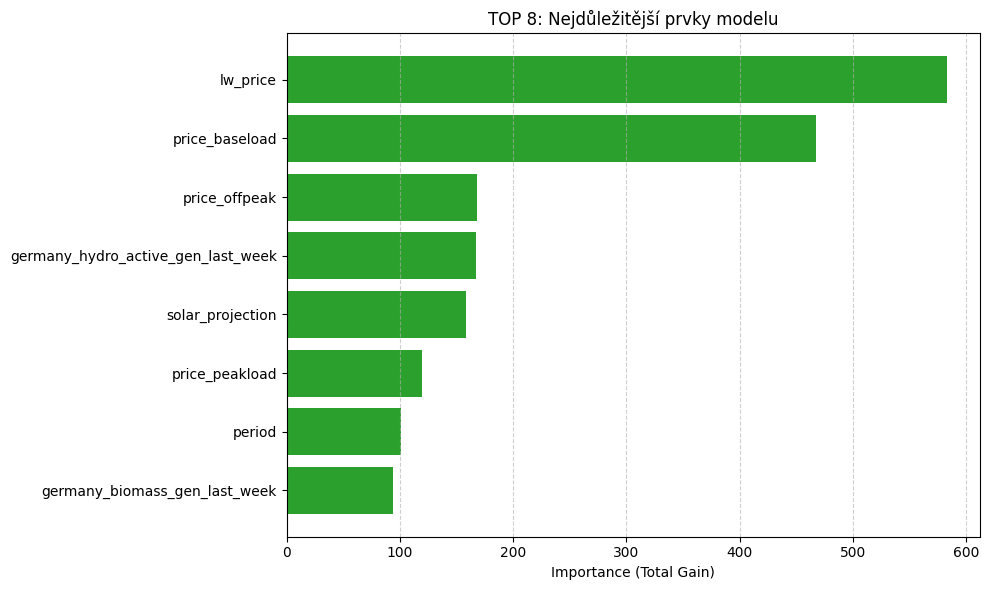
\includegraphics[width=0.95\linewidth]{images/important-features.jpg}
    \caption{Nejdůležitější příznaky}
    \label{fig:imporant-features}
\end{figure}

\begin{figure}[htbp]
    \centering
    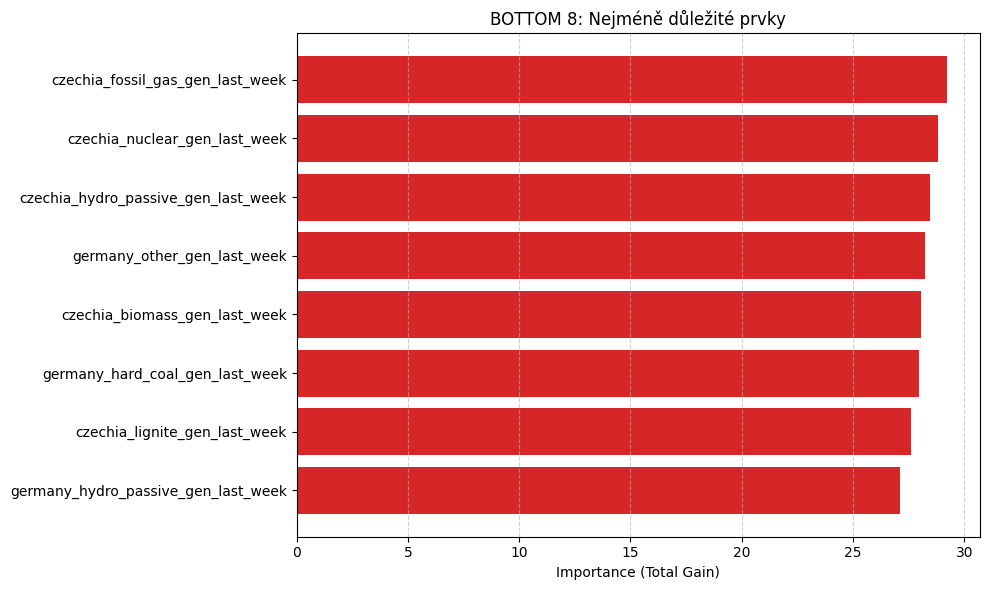
\includegraphics[width=0.95\linewidth]{images/useless_features.jpg}
    \caption{Nejméně důležité příznaky}
    \label{fig:useless-features}
\end{figure}

Mezi absolutní špičku (Top 8) se logicky zařadily cenové a~časové fundamenty. Nejsilnějším prediktorem byla cena přesně před týdnem (\texttt{lw\_price}), následovaná denními průměry \\(\texttt{price\_baseload}, \texttt{price\_offpeak}, \texttt{price\_peakload}). Extrémně vysoké hodnocení získala i~vlastní odvozená proměnná \\ \texttt{solar\_projection}, což potvrdilo smysluplnost provedeného Feature Engineeringu. Z~časových údajů se ukázala jako klíčová samotná čtvrthodina uvnitř dne (\texttt{period} 1--96).

Velmi cenným zjištěním byla pozice zpožděné výroby německých přečerpávacích elektráren (\texttt{germany\_hydro\_active\_gen\_last\_week}). Tyto zdroje fungují čistě na tržním principu arbitráže (nakupují levně, prodávají draze), a~jejich aktivita tak modelu poskytuje naprosto přesný signál o~napětí v~síti. Naopak vysoké umístění německé biomasy (\texttt{germany\_biomass}) bylo na základě doménové znalosti vyhodnoceno jako anomálie a~náhodná korelace bez reálné kauzality. Aby nedošlo k~zanesení šumu, byl tento příznak z~finálního datasetu manuálně odstraněn.

Pohled na opačný konec spektra (nejméně důležité příznaky) vedl k~radikálnímu prořezání matice. Ukázalo se, že zpožděné hodnoty výroby z~tradičních zdrojů, jako jsou české a~německé hnědouhelné či černouhelné elektrárny, modelu nepřinášejí žádnou informační hodnotu. Důvodem je jejich provoz v~základním zatížení~-- nevysvětlují krátkodobou volatilitu, na kterou cílíme. Z~tohoto důvodu byly z~datasetu odstraněny zcela všechny zpožděné příznaky tradičních zdrojů s~výjimkou vysoce flexibilních přečerpávacích a~akumulačních vodních elektráren v~Česku i~Německu.

\subsection{Teoretický popis zvolených algoritmů}
Pro vytvoření robustního prediktivního systému byly zvoleny dva odlišné algoritmické přístupy. Prvním z~nich je tradiční lineární regrese, která slouží jako tzv. \textit{baseline} (referenční model). Druhým je pokročilý stromový algoritmus XGBoost, který představuje hlavní výpočetní sílu celého řešení.

\subsubsection{Lineární regrese (Linear Regression)}
Jako referenční model pro porovnání výkonnosti byla zvolena standardní implementace lineární regrese z~knihovny Scikit-learn (\texttt{LinearRegression}). Tento základní statistický model předpokládá lineární vztah mezi cílovou proměnnou (cenou elektřiny) a~nezávislými příznaky. Algoritmus se snaží proložit vícerozměrným prostorem dat optimální nadrovinu tak, aby minimalizoval součet čtverců chyb (metoda nejmenších čtverců). Matematicky lze tento vztah zapsat jako:
$$ y = \beta_0 + \beta_1 x_1 + \beta_2 x_2 + \dots + \beta_n x_n + \epsilon $$
kde $y$ je predikovaná cena, $\beta_0$ je absolutní člen (intercept), $\beta_i$ jsou modelem naučené váhy jednotlivých fundamentů $x_i$ a~$\epsilon$ představuje náhodnou chybu. Výhodou tohoto modelu je jeho naprostá jednoduchost a~interpretabilita~\cite{hands-on-ml}. Zásadní nevýhodou na trhu s~elektřinou je však jeho neschopnost zachytit složité nelineární jevy a~skokové změny.

\subsubsection{XGBoost (Extreme Gradient Boosting)}
\label{subsubsec:xgboost}
Pro překonání limitů lineární regrese byl nasazen algoritmus XGBoost. Základním stavebním kamenem tohoto modelu je \textit{rozhodovací strom} (Decision Tree), přesněji řečeno regresní strom. Tento jednoduchý model funguje tak, že postupně štěpí vstupní prostor dat na základě série logických podmínek (například: \textit{Je hodina větší než 18?} nebo \textit{Je očekávaná výroba větru v~Německu nižší než 5000 MW?}). Na konci každé větve (v~tzv. listu) pak strom přiřadí konkrétní predikovanou hodnotu~\cite{hands-on-ml}. Jeden samotný strom je však pro komplexní energetický trh příliš slabý a~náchylný k~přeučení (overfitting).

XGBoost proto nevyužívá pouze jeden strom, ale staví tzv. ansámbl (les) stovek sekvenčně řazených stromů pomocí techniky \textbf{Gradient Boosting}~\cite{hands-on-ml}. Klíčovou myšlenkou tohoto přístupu je postupné učení z~vlastních chyb. 
Proces probíhá iterativně:
\begin{enumerate}
    \item První strom vytvoří základní, velmi hrubou predikci ceny (často jen průměrnou hodnotu).
    \item Následně se vypočítají rezidua (chyby), tedy rozdíly mezi skutečnou cenou a~predikcí prvního stromu.
    \item Druhý strom již nepredikuje samotnou cenu elektřiny, ale učí se predikovat právě tato rezidua~-- snaží se tedy opravit chybu prvního stromu.
    \item Třetí strom opravuje chyby, které zbyly po spojení prvního a~druhého stromu, a~takto proces pokračuje dále, dokud se chyba neustálí.
\end{enumerate}

Přívlastek \textit{Extreme} v~názvu algoritmu odkazuje na jeho pokročilé matematické a~softwarové optimalizace. Na rozdíl od tradičních boosting metod implementuje XGBoost silnou penalizaci složitosti stromů~\cite{xgboost} (tzv. L1 a~L2 regularizaci), čímž efektivně zabraňuje přeučení na historický šum. Zároveň disponuje nativní schopností zpracovávat chybějící hodnoty, pro které při tréninku automaticky vyhledává optimální směr štěpení. Právě tato kombinace robustnosti a~schopnosti modelovat vysoce nelineární interakce z~něj činí průmyslový standard pro predikci časových řad.

\subsection{Vyhodnocení výkonnosti a~srovnání modelů}
Pro objektivní posouzení kvality predikcí byla jako hlavní metrika zvolena Střední absolutní chyba (MAE~-- Mean Absolute Error). Její výpočet je dán vztahem:
$$ \text{MAE} = \frac{1}{n} \sum_{i=1}^{n} |y_i - \hat{y}_i| $$~\cite{hands-on-ml}
Tato metrika byla vybrána pro svou vysokou byznysovou výpovědní hodnotu, neboť vyjadřuje průměrnou odchylku predikce od skutečnosti přímo v~eurech za megawatthodinu (EUR/MWh).

Výsledky testování na neviděných datech (v~rámci chronologické křížové validace) potvrdily teoretické předpoklady. Referenční model lineární regrese dosáhl průměrné chyby zhruba 16~EUR/MWh. Na dynamický a~často extrémně volatilní trh s~elektřinou byla jeho statická povaha nedostatečná.

Po nasazení a~hyperparametrickém ladění algoritmu XGBoost došlo k~výraznému zpřesnění predikcí. Model dokázal stlačit chybovost na úroveň 13~EUR/MWh, čímž lineární regresi s~přehledem překonal. XGBoost exceloval především v~predikcích nočních hodin (baseload). 

\subsubsection{Problém večerní špičky}
Při hlubší analýze odchylek bylo zjištěno, že oba modely systematicky narážejí na identický problém: predikci cen ve večerních hodinách (typicky mezi 18:00 a~20:00). Zatímco celodenní průměrná chyba algoritmu XGBoost činila 13~EUR/MWh, v~tomto specifickém časovém okně se hodnota MAE běžně vyšplhala i~přes hranici 30~EUR/MWh. V~této době totiž prudce klesá výroba solárních elektráren a~zároveň raketově roste spotřeba domácností, do kterých se lidé vracejí z~práce.

\begin{figure}[htbp]
    \centering
    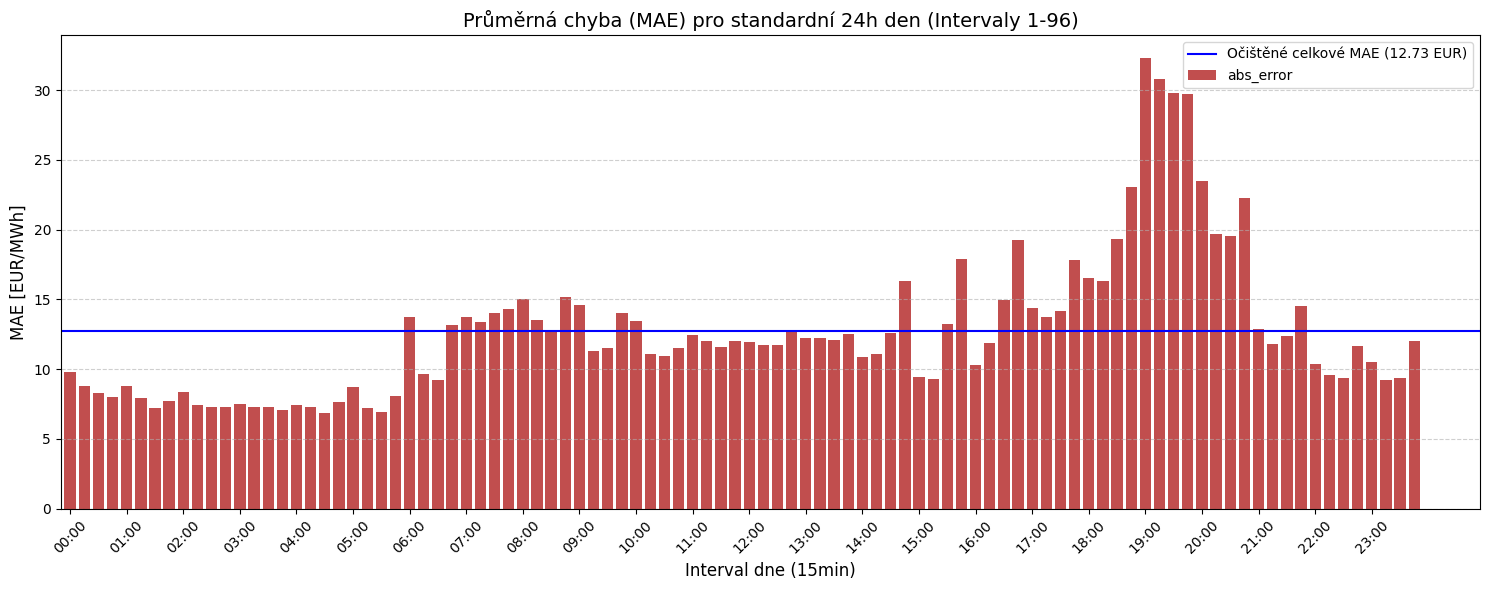
\includegraphics[width=1\linewidth]{images/mae_chart.png}
    \caption{Průměrná odchylka pro každou čtvrthodinu}
    \label{fig:mae-chart}
\end{figure}

V~těchto hodinách dochází na burze k~největší nervozitě a~k~těžko předvídatelným cenovým skokům, které často závisí na nepublikovaných obchodních strategiích velkých hráčů či náhlých výpadcích konvenčních bloků. Extrémní nárůst chybovosti modelu v~tomto okně jasně dokazuje, že chování trhu v~absolutní špičce již nelze plně vysvětlit pouze pomocí veřejně dostupných \textit{Day-Ahead} fundamentů a~k~dosažení komerční přesnosti by systém vyžadoval prémiová, vysokofrekvenční data.

\newpage
\section{Automatizace systému}
Zatímco fáze trénování a~evaluace modelu probíhala na statickém historickém datasetu, hlavním cílem práce bylo vytvořit živý, plně automatizovaný systém. Pro úspěšný přechod z~laboratorních podmínek do produkčního prostředí bylo nutné vyřešit architekturu každodenního běhu a~zajistit spolehlivý přísun aktuálních předpovědních dat pro nadcházející den (Day-Ahead).

\subsection{Spot Renewables: předpověď obnovitelných zdrojů}
\label{subsec:spot-renewables}
Aby mohl algoritmus XGBoost predikovat ceny na zítřejší den, musí mu být do vstupní matice dodány fundamenty platné pro zítřek~-- především očekávaná výroba z~větrných a~solárních elektráren v~Německu. Historická data ze systému SMARD již v~tomto bodě nedostačovala, neboť systém potřeboval meteorologický výhled do budoucnosti.

V~souladu se sekundární motivací práce (využít výhradně bezplatné veřejné zdroje) byla do automatizované pipeline integrována platforma \textit{Spot Renewables}~\cite{spot-renewables}. Tento portál poskytuje volně přístupné denní predikce generace z~obnovitelných zdrojů. Bezplatný přístup je však na této platformě zatížen významnou granularitní limitací: data nejsou poskytována v~požadovaném 15minutovém rozlišení, ale pouze v~agregované formě pro základní denní bloky (Baseload, Peakload a~Offpeak).

Tento nedostatek vysokofrekvenčních dat byl algoritmicky vyřešen pomocí syntetických projekcí (viz podkapitola \ref{subsec:odvozene-priznaky}). Systém v~produkci stáhne ze Spot Renewables agregovaný zítřejší výhled (např. solární Baseload) a~následně jej poměrově aplikuje na přesný 15minutový profil výroby z~minulého týdne. Tímto přístupem se podařilo překlenout bariéru placených meteorologických rozhraní a~poskytnout modelu kvalitní, i~když odvozený, Day-Ahead fundament.

\subsection{Integrace tržních očekávání z~burzy EEX}
Zatímco platformy jako ENTSO-E či Spot Renewables zásobují systém fyzikálními fundamenty (očekávaná spotřeba), pro přesnou cenovou predikci je neméně důležité znát i~aktuální finanční sentiment trhu. Tento sentiment nejlépe reflektují krátkodobé deriváty a~futures kontrakty. Jako primární zdroj těchto makroekonomických indikátorů byla do systému integrována lipská burza EEX (European Energy Exchange)~\cite{eex}, která je centrálním tržištěm pro evropskou energetiku.

V~rámci automatizovaného sběru dat jsou z~EEX stahovány aktuální ceny futures kontraktů pro základní zatížení (\textit{Baseload}) a~špičkové zatížení (\textit{Peakload}). Dále jsou z~této platformy získávány nejaktuálnější hodnoty emisních povolenek (EUA), které definují variabilní náklady fosilních zdrojů.

Získání cen pro Baseload a~Peakload sice pokrývá hlavní část trhu, nicméně pro modelování nočních propadů cen bylo žádoucí explicitně definovat i~cenu mimospičkovou (\textit{Offpeak}). Jelikož tuto hodnotu burza v~daném formátu přímo neposkytuje, bylo přistoupeno k~jejímu analytickému odvození.

Matematicky je denní Baseload (24 hodin) váženým průměrem Peakloadu (12 hodin, typicky 8:00--20:00) a~Offpeaku (zbylých 12 hodin). Cenu mimospičkového pásma tak lze pro každý den exaktně dopočítat jednoduchou algebraickou úpravou:
$$ \text{Offpeak} = 2 \times \text{Baseload} - \text{Peakload} $$

Tento výpočet byl implementován přímo do datové pipeline. Model tak pro každý predikovaný den získá kompletní trojici tržních indikátorů (Baseload, Peakload, Offpeak) i~přesnou cenu uhlíku (EUA), což mu umožňuje mnohem lépe ukotvit své predikce v~realitě aktuálního ekonomického prostředí.

\subsection{Objektová architektura a~automatizované spouštění}
Časování celého systému je striktně podřízeno pravidlům evropského denního trhu s~elektřinou (OTE). Brány trhu (tzv. Gate Closure) se pro obchodování na nadcházející den uzavírají přesně ve 12:00 CET. Aby měla predikce reálný komerční význam, musí být vypočtena a~doručena před tímto deadlinem.

Z~hlediska softwarového inženýrství je celý systém navržen plně 
objektově (OOP). Pro každý externí datový zdroj (OTE, ENTSO-E, EEX, Spot Renewables) byla naimplementována Python třída. 

Společným jmenovatelem těchto tříd je jejich konstruktor (\texttt{\_\_init\_\_}), který jako primární argument přijímá parametr \texttt{target\_date} (cílové datum). Tento přístup zajišťuje vysokou modularitu kódu~-- identické třídy lze bez úprav využít jak pro každodenní produkční stahování aktuálních dat, tak pro zpětné hromadné dotahování historie.

\begin{lstlisting}[language=Python, caption={Ukázka třídy pro datový zdroj}]
class OteFetcher:
    def __init__(self, date_input):
        if isinstance(date_input, datetime):
            self.target_date = date_input
        else:
            self.target_date = datetime.strptime(date_input, '%Y-%m-%d')
            
        self.date_str = self.target_date.strftime('%Y-%m-%d')
        
        self.url_ele = "https://www.ote-cr.cz/cs/kratkodobe-trhy/elektrina/denni-trh/@@chart-data"
        self.url_gas = "https://www.ote-cr.cz/cs/kratkodobe-trhy/plyn/vnitrodenni-trh/@@chart-data"
    #...zbytek tridy
\end{lstlisting}

Životní cyklus modelu v~produkčním prostředí je řízen systémovými plánovači (Cron) a~probíhá ve dvou oddělených fázích, které si popíšeme v~následujících kapitolách.

\newpage
\subsubsection{Prediktivní běh (každý den v~11:30 CET)}
Tento 30minutový předstih před uzavřením trhu představuje optimální okno, 
kdy již většina platforem publikovala své ranní výhledy na zítřek.
\begin{itemize}
    \item \textbf{Sběr dat:} Systém inicializuje instance jednotlivých datových tříd s~parametrem \texttt{target\_date} nastaveným na zítřejší den ($t+1$). Paralelně se stahují meteorologické a~fyzikální výhledy (Spot Renewables, ENTSO-E) i~aktuální finanční sentiment z~burzy (EEX futures a~povolenky EUA).
    \item \textbf{Předzpracování a~predikce:} Stažená data jsou sloučena do unifikované matice, a~aplikuje se Feature Engineering (např. výpočet solární projekce). Následně je sestavený vektor 96 čtvrthodin předán natrénovanému modelu XGBoost.
    \item \textbf{Uložení:} Vypočtené cenové predikce pro nadcházející den jsou uloženy do databáze a~okamžitě zpřístupněny pro uživatelské rozhraní.
\end{itemize}

\subsubsection{Evaluační běh (každý den ve 13:15 CET)}
Pro kontinuální sledování výkonnosti modelu byl zaveden druhý automatizovaný proces. Krátce po 13. hodině jsou již oficiálně známy a~publikovány skutečné zúčtovací ceny denního trhu pro zítřejší den. Skript ve 13:15 proto iniciuje třídu pro komunikaci s~OTE, tyto reálné (vyhlášené) ceny stáhne a~v~databázi je spáruje s~hodnotami, které systém sám predikoval v~11:30. Díky této zpětné vazbě lze v~reálném čase automaticky vyhodnocovat přesnost modelu (např. počítat denní MAE) a~okamžitě vizualizovat případné odchylky na trhu.

\subsection{Návrh databázové vrstvy}
Jakmile automatizované skripty (Cron Jobs) dokončí fázi inferenčních výpočtů či stahování reálných dat, je nezbytné výsledky trvale a~bezpečně uložit. Pro perzistenci dat a~jejich následné zpřístupnění uživatelskému rozhraní byla zvolena relační databáze, která zajišťuje integritu a~rychlé dotazování.

Struktura databáze byla navržena s~ohledem na maximální efektivitu a~minimalizaci redundance. Vzhledem k~povaze časových řad na denním trhu byla vytvořena centrální tabulka \texttt{price\_predictions}, která sdružuje jak predikované, tak skutečné vyhlášené hodnoty.

Klíčovým inženýrským rozhodnutím při návrhu schématu bylo použití složeného primárního klíče. Tento klíč je tvořen kombinací cílového data (\texttt{delivery\_date}) a~konkrétní čtvrthodiny (\texttt{period}). Toto řešení nativně zabraňuje vzniku duplicitních záznamů pro stejný interval a~zároveň bez problému pojme kalendářní anomálie, jako je den se 100 periodami při přechodu na zimní čas.

\begin{lstlisting}[language=SQL, caption={SQL schéma pro ukládání predikcí a~reálných cen se složeným primárním klíčem}]
CREATE TABLE IF NOT EXISTS price_predictions (
    delivery_date DATE,
    period INTEGER,               
    predicted_price DECIMAL(10, 2),
    actual_price DECIMAL(10, 2),   
    PRIMARY KEY (delivery_date, period) 
);
\end{lstlisting}
Běh systému pak v~praxi vypadá následovně: Prediktivní pipeline v~11:30 vloží do tabulky nové řádky s~vyplněným datem, periodou a~predikovanou cenou (přičemž sloupec \texttt{actual\_price} zůstává prázdný). Následný evaluační běh ve 13:15 pak tyto existující záznamy pouze aktualizuje (operace \textit{UPDATE}) o~oficiální burzovní výsledky.

\newpage
\section{Uživatelské rozhraní}
Aby byl celý prediktivní systém plně využitelný v~praxi, byla nad databázovou vrstvou vybudována lehká webová aplikace (Dashboard). Jejím primárním cílem je poskytnout uživateli okamžitý vizuální přehled o~očekávaném vývoji cen na denním trhu a~umožnit interaktivní zpětné vyhodnocování historické přesnosti modelu.

Z~hlediska softwarové architektury byl kladen důraz na minimalismus, vysoký výkon a~snadnou údržbu. Namísto robustních frontendových frameworků byla zvolena moderní a~vysoce efektivní kombinace technologií:

\begin{itemize}
    \item \textbf{Backend (Flask):} Jako aplikační server byl využit 
    odlehčený mikro-framework Flask v~jazyce Python. Jeho úkolem je 
    přijímat požadavky od uživatele, dotazovat se do databáze 
    (\texttt{price\_predictions}) na konkrétní datum a~vracet 
    vyrenderované HTML šablony.
    
    \item \textbf{Styling (Tailwind CSS):} Pro zajištění responzivního 
    a~moderního designu byl použit framework Tailwind CSS. 
    Umožnil rychlou tvorbu čistého uživatelského prostředí bez nutnosti 
    psát a~spravovat oddělené kaskádové styly.
    
    \item \textbf{Interaktivita (HTMX):} Pro plynulý uživatelský zážitek, 
    například při změně prohlíženého data, byla využita knihovna HTMX. 
    Ta umožňuje provádět asynchronní AJAX požadavky a~dynamicky 
    přepisovat pouze relevantní části stránky bez 
    nutnosti kompletního znovunačtení celého webu.
    
    \item \textbf{Vizualizace (Google Charts):} Samotné vykreslení 
    96 čtvrthodinových intervalů zajišťuje knihovna Google Charts. 
    V~přehledném spojnicovém grafu jsou přes sebe vyneseny křivky 
    predikované ceny (\textit{Predicted}) a~skutečné burzovní ceny 
    (\textit{Actual}), což umožňuje vizuálně identifikovat případné 
    odchylky ve večerních špičkách.
\end{itemize}

Kromě samotné vizualizace trendů poskytuje rozhraní denní přehled, který se nachází bezprostředně pod grafem. Tento panel dynamicky počítá denní statistiky a~nabízí uživateli hlubší vhled do výkonnosti 
modelu v~daném dni. Panel obsahuje následující metriky:
\begin{itemize}
    \item \textbf{Průměrná odchylka (MAE):} Udává celkovou absolutní chybovost modelu v~průběhu celého dne.
    \item \textbf{Mediánová chyba:} Slouží jako robustní metrika, která (na rozdíl od průměru) není zkreslena několika extrémními výkyvy během večerní špičky.
    \item \textbf{Systematické zkreslení (Bias):} Kvantifikuje, zda měl model v~daný den tendenci trh plošně nadhodnocovat (pozitivní bias), či naopak podhodnocovat (negativní bias).
\end{itemize}

\begin{figure}[htbp]
    \centering
    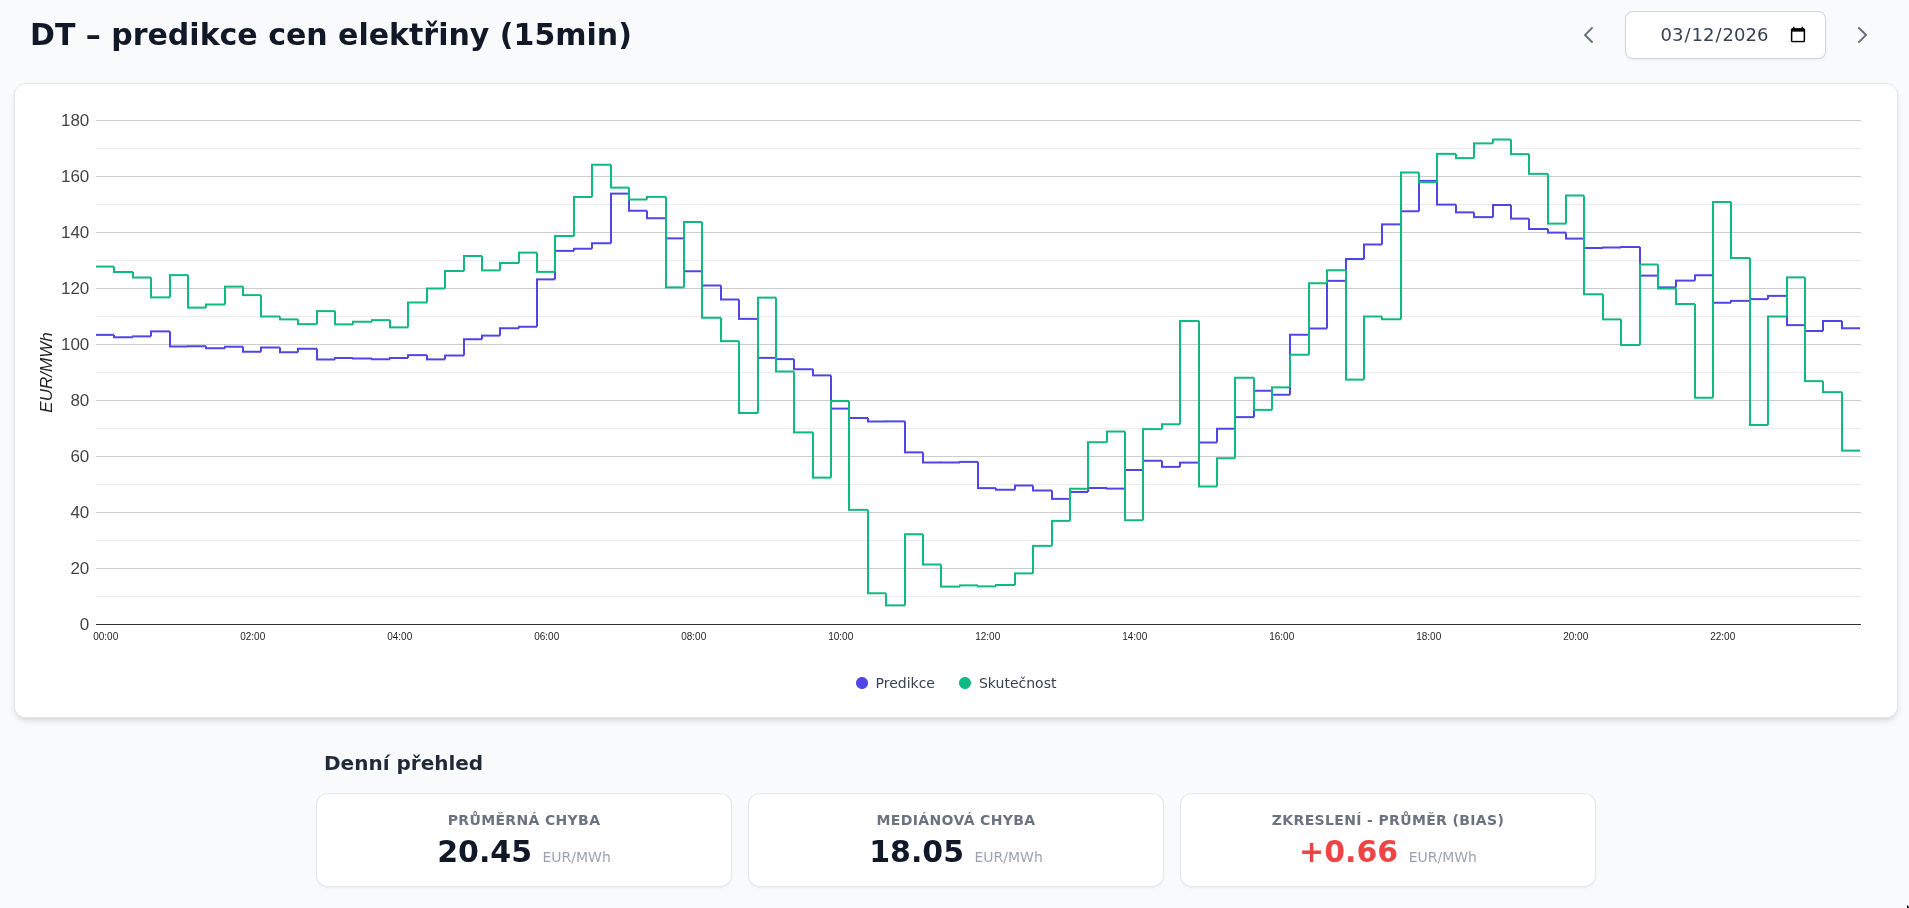
\includegraphics[width=1\linewidth]{images/ui-example-1.jpg}
    \caption{Ukázka uživatelského rozhraní}
    \label{fig:ui-example-1}
\end{figure}

\newpage
Pro další diagnostiku má uživatel možnost rozkliknout si přehled jednotlivých period. V~tomto zobrazení je pro každou konkrétní 15minutovku explicitně vyčíslena predikovaná cena, skutečná cena a~jejich přesná odchylka. To umožňuje analytikovi přesně identifikovat časové úseky, ve kterých model ztratil korelaci s~realitou trhu.

\begin{figure}[htbp]
    \centering
    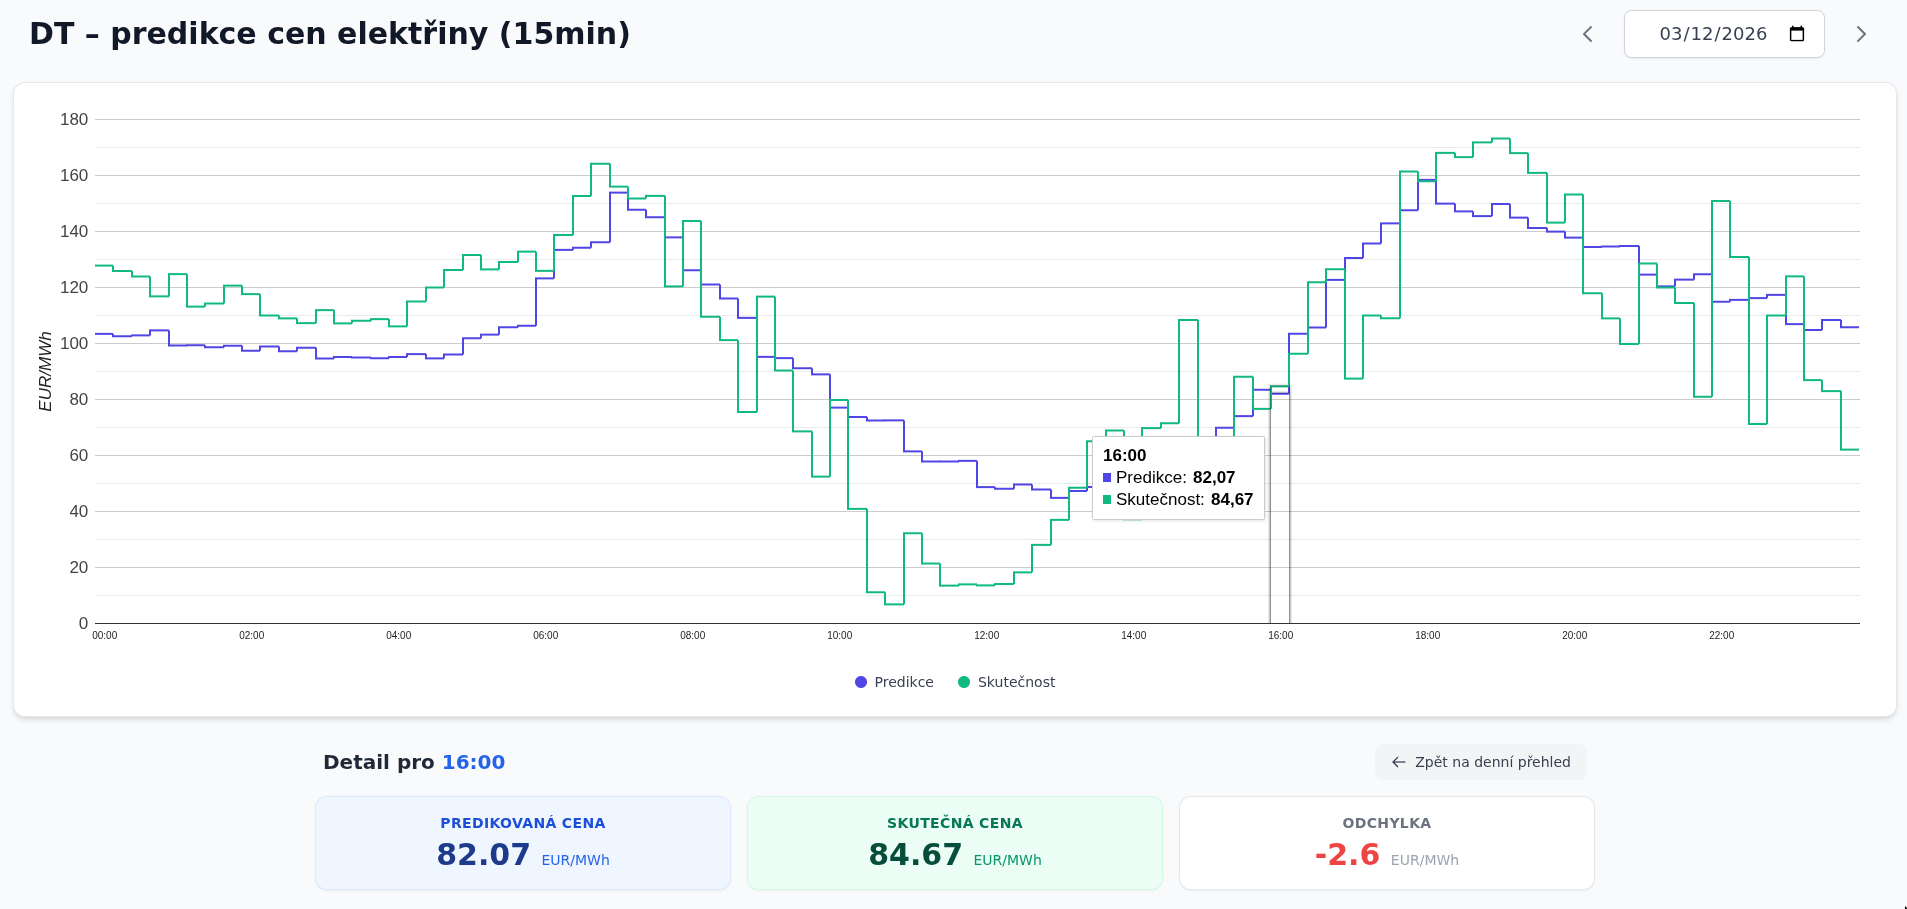
\includegraphics[width=1\linewidth]{images/ui-example-2.jpg}
    \caption{Ukázka detailu periody}
    \label{fig:ui-example-2}
\end{figure}

Tato architektura uzavírá celý životní cyklus dat. Systém zcela autonomně stahuje fundamenty, provádí výpočty v~XGBoostu, ukládá je do relační databáze a~prostřednictvím rychlého webového rozhraní je prezentuje koncovému uživateli v~intuitivní grafické podobě.

\newpage
\section{Závěr}
Hlavním cílem této práce bylo navrhnout, implementovat a~otestovat komplexní end-to-end systém pro predikci cen elektřiny na českém denním trhu. Jak bylo naznačeno v~úvodu, projekt si kladl za cíl vyzkoušet vývoj modelu na problému z~reálného světa a~ověřit možnosti i~limity strojového učení postaveného výhradně na veřejně dostupných bezplatných datech.

Dosažená přesnost modelu logicky nedosahuje absolutní dokonalosti drahých komerčních systémů, za kterými stojí rozsáhlé týmy analytiků a~prémiová meteorologická data. Tento výsledek však přesně reflektuje a~potvrzuje testovaný limit bezplatných zdrojů. I~přes tato omezení se algoritmu XGBoost podařilo úspěšně zachytit klíčové nelineární závislosti a~základní logiku trhu, čímž systém prokázal svou vysokou analytickou hodnotu.

Nejvýznamnějším zjištěním a~přínosem celého projektu je potvrzení faktu, že při vývoji umělé inteligence pro reálné nasazení často nepředstavuje největší výzvu samotný výběr a~ladění algoritmu, ale sběr, čištění a~synchronizace surových dat. Práce se nespokojila s~pouhým trénováním modelu v~ideálních laboratorních podmínkách na předem připraveném datasetu, ale postavila reálnou a~odolnou datovou architekturu. Úspěšně tak byly vyřešeny komplexní inženýrské problémy, jako jsou datové anomálie spojené s~přechodem na letní a~zimní čas nebo algoritmické doplňování chybějících víkendových záznamů z~finančních burz.

Výsledkem tohoto úsilí je plně funkční, automatizovaná datová pipeline zakončená interaktivním webovým rozhraním. Vytvořený systém neslouží pouze jako akademická ukázka, ale funguje jako robustní a~stabilní základ, na kterém lze v~budoucnu dále stavět~-- například budoucí integrací placených datových zdrojů. Projekt tak úspěšně naplnil všechny stanovené cíle a~jasně demonstroval obrovský potenciál aplikované datové analytiky v~současné energetice.

\subsection{Možnosti budoucího rozvoje}
Vytvořená softwarová a~datová architektura představuje robustní základ, který je díky svému objektovému návrhu připraven na další rozšiřování. Pro budoucí iterace a~případné nasazení systému do reálného komerčního prostředí se nabízejí tři hlavní směry technického a~analytického rozvoje.

\subsubsection{Automatizované přetrénování modelu}
V~současné podobě je model XGBoost natrénován staticky na historickém datasetu a~v~produkci provádí pouze každodenní predikce. Vzhledem k~dynamické povaze energetického trhu, kde se neustále mění vzorce chování, by dalším logickým krokem byla implementace plně automatizovaného přetrénování. Systém by mohl například na týdenní bázi automaticky rozšířit svou trénovací matici o~čerstvě nasbíraná reálná data, model přetrénovat, vyhodnotit jeho novou přesnost a~nasadit ho do produkce. Tím by se prediktivní jádro dokázalo plynule adaptovat na měnící se makroekonomické i~sezónní podmínky.

\subsubsection{Detailní meteorologická data}
Jak potvrdila analýza odchylek u~večerních špiček, jedním z~limitů modelu je absence detailních vysokofrekvenčních dat o~lokálním počasí. Tento nedostatek lze efektivně vyřešit obohacením datasetu o~další meteorologické proměnné. Zahrnutí parametrů, jako je lokální teplota, oblačnost či rychlost větru, by modelu poskytlo mnohem přesnější základ pro odhad reálné spotřeby a~výroby. Vysoce perspektivním příznakem pro budoucí vývoj je například UV index. Ten představuje vynikající a~přímý indikátor reálného výkonu solárních elektráren, jehož integrace v~15minutovém rozlišení by s~největší pravděpodobností výrazně snížila chybovost systému během výkyvů.

\subsubsection{Experimenty s~neuronovými sítěmi (Deep Learning)}
Ačkoliv algoritmus XGBoost v~této práci prokázal vynikající výsledky, jeho přirozeným limitem je fakt, že mu paměť musíme dodávat uměle pomocí manuálně vytvořených zpožděných příznaků (Lag Features). Zajímavým směrem dalšího vývoje by proto byl přechod k~pokročilým neuronovým sítím, které jsou navrženy tak, aby časové souvislosti chápaly přirozeně. Takový model by se nedíval na data jako na izolované řádky v~tabulce, ale vnímal by je jako souvislý příběh. Dokázal by si tak sám „všimnout“ trendů a~cyklů, které lidskému oku i~stromovým algoritmům mohou uniknout, což by mohl být klíč k~ještě přesnějšímu zachycení extrémních cenových výkyvů.

\newpage
\begin{thebibliography}{40}
\bibitem{entsoe} ENTSO-E. \textit{ENTSO-E Transparency Platform}. Online. 2026. Dostupné z: https://transparency.entsoe.eu/. [cit. 2026-03-13].

\bibitem{merit-order} NANO ENERGIES. \textit{Merit order}. Online. 2026. Dostupné z: https://nanoenergies.cz/slovnik/merit-order. [cit. 2026-03-13].

\bibitem{ote-kratkodobe-trhy} OTE, A.S. \textit{Krátkodobé trhy}. Online. 2026. Dostupné z: https://www.ote-cr.cz/cs/kratkodobe-trhy/elektrina/parametry-kratkodobych-trhu. [cit. 2026-03-13]. 

\bibitem{ote-dt-vysledky} OTE, A.S. \textit{Výsledky denního trhu ČR -- 14.~03.~2026}. Online. 2026. Dostupné z: https://www.ote-cr.cz/cs/kratkodobe-trhy/elektrina/denni-trh?time\_resolution=PT15M\&date=2026-03-14. [cit. 2026-03-13].

\bibitem{jupyter} JUPYTER. \textit{Jupyter}. Online. 2026. Dostupné z: https://jupyter.org/. [cit. 2026-03-14].

\bibitem{pandas-docs} PANDAS. \textit{Pandas documentation}. Online. 2026. Dostupné z: https://pandas.pydata.org/docs/. [cit. 2026-03-14].

\bibitem{pandas-dataframe} PANDAS. \textit{Pandas DataFrame}. Online. 2026. Dostupné z: https://pandas.pydata.org/docs/reference/frame.html. [cit. 2026-03-14].

\bibitem{numpy-docs} NUMPY. \textit{NumPy documentation}. Online. 2026. Dostupné z: https://numpy.org/doc/stable/. [cit. 2026-03-14].

\bibitem{numpy-ndarray} NUMPY. \textit{NumPy ndarray}. Online. 2026. Dostupné z: https://numpy.org/doc/stable/reference/arrays.ndarray.html. [cit. 2026-03-14].

\bibitem{scikit-learn} SCIKIT-LEARN. \textit{Scikit-Learn}. Online. 2026. Dostupné z: https://scikit-learn.org/. [cit. 2026-03-14].

\bibitem{linear-regression} SCIKIT-LEARN. \textit{sklearn.linear\_model}. Online. 2026. Dostupné z: https://scikit-learn.org/stable/api/sklearn.linear\_model.html. [cit. 2026-03-14].

\bibitem{xgboost} XGBOOST. \textit{XGBoost Documentation}. Online. 2025. Dostupné z: https://xgboost.readthedocs.io/. [cit. 2026-03-14].

\bibitem{matplotlib} MATPLOTLIB. \textit{API Reference}. Online. 2026. Dostupné z: https://matplotlib.org/stable/api/index. [cit. 2026-03-14].

\bibitem{postgres} THE POSTGRESQL GLOBAL DEVELOPMENT GROUP. \textit{PostgreSQL: The World's Most Advanced Open Source Relational Database}. Online. 2026. Dostupné z: https://www.postgresql.org/. [cit. 2026-03-14].

\bibitem{flask} PALLETS. Flask. Online. 2010. Dostupné z: https://flask.palletsprojects.com/. [cit. 2026-03-14]. 

\bibitem{apscheduler} ALEX GRÖNHOLM. Advanced Python Scheduler. Online. 2009. Dostupné z: https://apscheduler.readthedocs.io/. [cit. 2026-03-14]. 

\bibitem{docker} DOCKER INC. \textit{Docker}. Online. 2026. Dostupné z: https://www.docker.com/. [cit. 2026-03-14].

\bibitem{docker-compose} DOCKER INC. \textit{Docker Compose}. Online. 2026. Dostupné z: https://docs.docker.com/compose/. [cit. 2026-03-14].

\bibitem{tailwind} TAILWIND LABS INC. \textit{Tailwind CSS - Rapidly build modern websites without ever leaving your HTML}. Online. 2026. Dostupné z: https://tailwindcss.com/. [cit. 2026-03-14].

\bibitem{htmx} HTMX. \textit{HTMX - high power tools for html}. Online. 2026. Dostupné z: https://htmx.org/. [cit. 2026-03-14].

\bibitem{google-charts} GOOGLE. Charts. Online. 2026. Dostupné z: https://developers.google.com/chart. [cit. 2026-03-14].

\bibitem{ote-rocni-zprava} OTE, A.S. \textit{Roční zpráva 2025}. Online. 2025. Dostupné z: https://www.ote-cr.cz/cs/statistika/rocni-zprava?date=2025-01-01. [cit. 2026-03-14]. 

\bibitem{smard-de} BUNDESNETZAGENTUR. \textit{SMARD}. Online. 2026. Dostupné z: https://www.smard.de/en. [cit. 2026-03-14].

\bibitem{entsoe-api} ENTSOE-E. \textit{Transparency Platform Restful API}. Online. 2026. Dostupné z: https://documenter.getpostman.com/view/7009892/2s93JtP3F6. [cit. 2026-03-14].

\bibitem{ceps} ČEPS, A.S. \textit{Zatížení soustavy}. Online. 2026. Dostupné z: https://www.ceps.cz/cs/data\#Load. [cit. 2026-03-14].

\bibitem{xml-parser} PYTHON SOFTWARE FOUNDATION. \textit{ElementTree XML API}. Online. 2026. Dostupné z: https://docs.python.org/3/library/xml.etree.elementtree.html. [cit. 2026-03-14].

\bibitem{python-requests} MMXVIX. A~KENNETH REITZ PROJECT. \textit{Requests: HTTP for Humans}. Online. 2026. Dostupné z: https://requests.readthedocs.io/. [cit. 2026-03-14].

\bibitem{oenergetice} OM SOLUTIONS S.R.O. \textit{Cena emisní povolenky (EUA)}. Online. 2026. Dostupné z: https://oenergetice.cz/energostat/ceny-aktualne/emisni-povolenka. [cit. 2026-03-14].

\bibitem{time-series-split} SCIKIT-LEARN. TimeSeriesSplit. Online. 2026. Dostupné z: https://scikit-learn.org/stable/modules/generated/sklearn.model\_selection\\.TimeSeriesSplit. [cit. 2026-03-15].

\bibitem{hands-on-ml} GÉRON, Aurélien. \textit{Hands-on Machine Learning with Scikit-Learn, Keras and TensorFlow}. 2. vydání. O'Reilly Media, 2017. ISBN 9781491962244.

\bibitem{spot-renewables} EUROWIND GMBH. \textit{Spot renewables}. Online. 2026. Dostupné z: https://www.spotrenewables.com/index.php?page=freeresources. [cit. 2026-03-15].

\bibitem{eex} EUROPEAN ENERGY EXCHANGE AG. \textit{Market Data Hub}. Online. 2026. Dostupné z: https://www.eex.com/en/market-data/market-data-hub. [cit. 2026-03-15].

\end{thebibliography}

\newpage
\listoffigures
\lstlistoflistings

\section*{Přílohy}
\addcontentsline{toc}{section}{Přílohy}
\begin{enumerate}
  \item Zdrojový kód -- online přístupný na \\ \texttt{https://github.com/freddycz/electricity-price-prediction-model}
\end{enumerate}

\end{document}